%%%%%%%%%%%%%%%%%%%%%%%%%%%%%%%%%%%%%%%%%%%%%%%%%%%%%%%%%
%    Formato de memoria de Trabajo Final de Grado (TFG) para la Facultad de Ingeniería de la Universidad Nacional de Asunción.

%   Version 2.0.1 por ProfMsc. Ing. Sergio Ramón Toledo Gallardo del 10 de junio de 2015                           
%- La compilación debe realizarse utilizando el comando pdflatex o pdflatexmk (para Mac)%
% Los programas necesarios son Miktex 2.9 (distribución latex) y algún procesador como el texmaks o texniccenter
%- Para texnicCenter Usar makeindex y habilitar usar bibtex
%-  Al imprimir el PDF se debe seleccionar tamaño real y Elegir origen por tamaño de pagina PDF para respetar los margenes requeridos   
%- Las figuras deben cargarse en la carpeta "imagenes" en formato pdf para optimizar la velocidad de compilación, sin embargo también se permiten formatos jpg y eps.
%- Las referencia bibliográficas se cargan en el archivo    fiuna.bib                                                       %%%%%%%%%%%%%%%%%%%%%%%%%%%%%%%%%%%%%%%%%%%%%%%%%%%%%
\documentclass[oneside, a4paper, 12pt]{fiuna}
\usepackage{fiuna}

%%%%%%%%%%%%%%%%%%%%%%%%%%%%%%%%%%%%%%%%%%%%%%%%%%%%%%%%%%
%               Inicio del documento                     %
%%%%%%%%%%%%%%%%%%%%%%%%%%%%%%%%%%%%%%%%%%%%%%%%%%%%%%%%%% 
\begin{document}

%%%Introduzca el nombre de los autores
\autor[Carlos Ozuna] {Carlos Buenaventura Ozuna Loncharich}
\autor[Oscar Valdez]{Oscar Bartolome Valdez Sarubbi}
%\autor{Autor 2}
%%%Introduzca el título del TFG
\titulo{Implementación de un ChatBot utilizando algoritmos de Inteligencia Artificial.}
%%%introduce la carrera
\carrera{Ingenier\'ia Electr\'onica}
%%%Nombre del Asesor del TFG %%%%%
\asesor{Ing. Asesor}
%\asesor{Ing. Asesor 2}
%\asesor{Ing. Asesor 3}
%%%%%%Ciudad donde se presenta%%%%%%%%%%%
\ciudad{San Lorenzo}
%%%%%% A quien se dedique %%%%%%%%%%%%%%
\dedicatoria{A quien se dedique}
\pagenumbering{roman}

\preliminares

\pagenumbering{arabic}
\tableofcontents
\listoffigures
\listoftables
%% En caso de no tener anexos comentar la siguiente linea
\listofappendices

\formatoTitulos

%%% Inician los capítulos de la memoria de TFG%%%%
%cada capitulo se introduce con \input
%El primer capitulo siempre es la introducción al TFG
%^--- El primer capítulo es fijo y siempre se llama introducción
\chapter[Introducción]{Introducción}
Durantee los últimos años, la Inteligencia Artificial (IA) ha tenido un crecimiento exponencial,
esto se debe principalmente a la capacidad de cómputo asequible y de alto rendimiento, además de
los grandes volúmenes de datos que se encuentran disponibles.\cite{Oracle}\\
\indent La IA tiene varias áreas de estudio, entre ellas se encuentra el Procesamiento de Lenguaje
Natural (NLP, por sus siglas en inglés), encargado de hacer que las computadoras entiendan e
interpreten el lenguaje humano con la ayuda de modelos estadísticos, machine learning y deep
learning.\\
\indent Una de las tantas aplicaciones prácticas del NLP son los chatbots, programas que imitan la
conversación humana.Los chatbots son capaces de interactuar con personas y de responder
adecuadamente a sus preguntas, son bastante accesibles, eficientes y de alta disponibilidad,
permitiendo así que distintas industrias se beneficien de el, entre las que destacan el comercio
electrónico, los seguros y el cuidado de la salud .\cite{building_chat-bots-with-python}\\
\indent En este trabajo se presenta un chatbot para el sector de la educación, donde el estudiante
pueda realizar sus consultas académicas y la respuesta deberá ser generada de acuerdo a ciertas
técnicas de coincidencia de patrones.

\section{Objetivo General}
Desarrollar e implementar un Chatbot utilizando algoritmos de Inteligencia Artificial (IA).

\section{Objetivos Específicos}
\begin{itemize}
	\item Comparar distintas Tecnologías para abordar el problema.
	\item Orientar el chatbot a dudas comunes de los estudiantes de la Facultad de Ingeniería en
	      atención al alumno.
	\item Recopilar, procesar y filtrar preguntas frecuentes para contar con un dataset propio.
	\item Seleccionar, entrenar y probar el algoritmo utilizando el dataset generado.
	\item Implementar el chatbot para su uso por estudiantes de la Facultad de Ingeniería
	\item Agregar una interfaz, propia o a una ya existente para el uso por los alumnos.
\end{itemize}

\section{Alcance y limitaciones}
Se pretende desarrollar un Chatbot que utilice algoritmos de inteligencia artificial para responder a preguntas
frecuentes de los alumnos de la Facultad de Ingeniería de la UNA. El entrenamiento de la IA se
llevará a cabo utilizando un dataset propio en conjunto con otros ya existentes.
Una previa comparativa entre distintas librerías y plataformas es necesaria para escoger la mejor
solución al objetivo planteado.

%Luego inican los demas capítulos
\chapter[Revisión de literatura]{Marco Teórico}

\subsection[Reseña Histórica]{Reseña Histórica}
Para empezar a adentrarnos a los conceptos del Procesamiento de Lenguaje Natural primero
empezaremos a repasar hitos importantes en áreas de conocimiento afines.
% https://www.cs.bham.ac.uk/~pjh/sem1a5/pt1/pt1_history.html
Los primera aplicación reconocida como una NPL fueron en 1948 que fue un buscador de palabras en el
diccionario de desarrollado en Birkbeck College de Londres por Warren Weaver. Luego rápidamente
surgió como idea de investigación crear una maquina de traducción automática en varios grupos de en
Estados Unidos, Reino Unido, Francia y Rusia. Los primeros grupos se concentraron en traducir texto
en Alemán, cuando los textos de la Segunda Guerra Mundial se volvieron obsoletos, pasaron a el Ruso
el mayor problema fue que no existían todavía fundamentos formales de al computación, ni mucho
menos de NLP. La mayoría de los investigadores eran matemáticos e inmigrantes bilingües que
intentaban encontrar relaciones entre ambos lenguajes. La investigación concluyo en que todavía no
existían los recursos necesarios para abordar dicho problema, pero se desarrollaron mejoras en
herramientas para la traducción asistida.\cite{hancox}
%  Sumit raj
En 1950 Alan Turing desarrolla el test de Turing que es un test para distinguir el nivel de
inteligencia de una maquina, propuso que un humano evaluara las conversaciones en un lenguaje
natural entre un humano y una máquina diseñada para dar respuestas similares a los humanos. Lo que
pudo definir la inteligencia de un sistema de computo de una forma comparable a la inteligencia
humana.
En el año 1954 un experimentó de colaboración de la Georgetown University e IBM se  hace publica la
primera demostración logra la traducción automática de mas de 60 se oraciones en Ruso al Ingles.
Las oraciones eran previamente elegidas que trataban de temas políticos, legales, matemáticos y
científicos. Luego eran ingresados a la maquina escritos en Ruso con letras romanizadas. El método
era principalmente lexicográfico basado en un diccionario de relaciones de palabras de ambos
idiomas.\cite{ibm_2003}
En las décadas posteriores se siguieron dando avances con métodos basados en reglas algorítmicas
como arboles de decisión para el procesamiento del lenguaje y la traducción automática. A partir de
los 2000s la investigación se centro en algoritmos de Machine Learning no supervisados y semi
supervisados, por amplia disponibilidad de información no clasificados en literatura e internet,
por lo general estos métodos son menos eficientes que los algoritmos supervisados pero la cantidad
de datos existentes pueden equiparar estas deficiencias. En la segunda década del nuevo milenio se
utilizaron nuevos métodos basados en Aprendizaje de características y Deep Learning lo que nos trae
al estado actual del arte que discutiremos en la siguiente sección.

\section[Procesamiento de lenguaje natural]{Procesamiento de lenguaje natural (NPL)}
El procesamiento de lenguaje natural o por sus siglas en inglés NPL(de natural language processing)
es un campo de las Ciencias de Computación y la Lingüística que trata con métodos para analizar,
modelar y entender el lenguaje humano.

%---usar sownya vajja Practical Natural Language Processing_ A Comprehensive Guide to Building Real como referencia

\subsection{Lenguaje}% que es un lenguaje, fonemas, syntaxis, etc 
Primero de los conceptos claves para poder adentrarnos a  NLP es definir el Lenguaje, un Lenguaje
es un sistema de comunicación que involucra una combinación compleja de componentes como, letras,
palabras, etc. La Lingüística es el estudio sistemático del lenguaje. Para poder estudiar NLP, es
importante entender componentes del lenguaje.\cite{sowmya_practical_npl}
\begin{figure}[h]
	\centering
	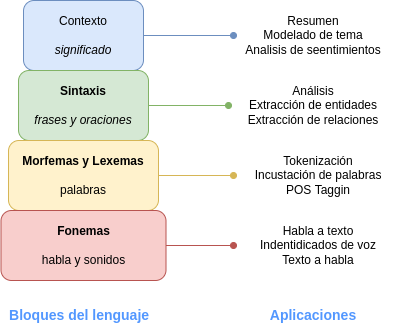
\includegraphics[width=\textwidth]{imagenes/Cap 2/lenguaje.drawio.png}
	\caption{Aplicaciones de partes de un Lenguaje}
	\label{fig:Arquitectura}
	\cite{sowmya_practical_npl}
\end{figure}

%metodos heuristicos
\subsection{Métodos Heurísticos y basado en reglas}

Similarmente a otros métodos primitivos usando AI, los primeros intentos en el diseño de sistemas
de NLP fueron
en construir reglas de acciones a manualmente por medio de arboles de decisión. Esto requiere que
lo desarrolladores tengan
experiencia en el dominio
del problema para formular las reglas que puedan ser incorporadas al programa.\\
En estos sistemas también se requieren recursos como diccionarios y tesauros, típicamente
compilados y digitalizado. Otra
herramienta muy poderosa en la implementación de sistemas basados en reglas son las Expresiones
Regulares(Regex por sus
siglas en ingles). Una expresión regular es un conjunto de caracteres o patrón que es utilizada
para coincidir y
encontrar subcadenas en un texto como
\verb|^([a-zA-Z0-9_\-\.]+)@([a-zA-Z0-9_\-\.]+)\.([a-zA-Z]{2,5})$|
que es utilizado encontrar direcciones de email validas en un texto.\\
Las reglas y heuristica juegan un rol importande en todo el ciclo de vida de proyectos de NLP
incluso hoy en dia. En un
por un lado, estos son una buena manera de desarrollar primeras versiones. O también pueden ser de
suma importancia en
sistemas basados en AI para llenar vacíos o limitaciones de los modelos probabilísticos.
\cite{sowmya_practical_npl}

%Metodos basados en ML
\subsection{Métodos basados en Aprendizaje Automático (Machine Learning)}
El Aprendizaje Automático o ML(por sus siglas en ingles) son aplicados para datos de texto así como
también son utilizados
en otro tipos de datos, como imágenes, voz y datos estructurados. Métodos de aprendizaje
supervisados como clasificación y
regresión con usados con mucha frecuencia en NLP. Como por ejemplo para buenas aplicaciones son par
clasificar temas de
artículos en el caso de calificadores.\\
Por otro lado las técnicas de regresión suelen ser utilizadas para dar una predicción numérica,
como por ejemplo el precio
de un stock basado en discusiones en una red social.Similarmente métodos no supervisados pueden ser
útiles para
agrupar documentos similares.
%deep learning
\subsection{Aprendizaje Profundo}

Aprendizaje profundo o Deep learning(DL) en ingles, es una evolución mas compleja de los algoritmos
de ML convencionales,
se trata de combinaciones de nodos que emulan el funcionamiento de las redes neuronales del
cerebro, sin entrar en mucho detalle procederemos a analizar los métodos basados en DL mas
utilizados y exitosos actualmente en el área de NLP.

\subsection{Redes Neuronales Recurrentes(RNN)}

En todos los lenguajes una oración tiene una dirección de lectura, por ejemplo en el Castellano se
lee de izquierda a derecha. Entonces un modelo que puede ser útil para leer progresivamente una
entrada de texto podría ser muy útil para NLP. Las Redes Neuronales recurrentes o RNNs por sus
siglas del ingles están específicamente diseñadas para mantener
un procesamiento secuencial y memoria de los pasos anteriores. Esta memoria es temporal y la
información es almacenada y
actualizada en cada paso de lectura de la RNN.

\begin{figure}[h]
	\centering
	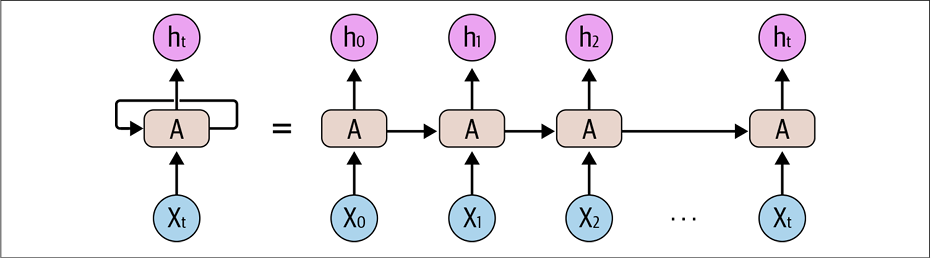
\includegraphics[width=\textwidth]{imagenes/Cap 2/rnn.png}
	\caption{Aplicaciones de partes de un Lenguaje}
	\label{fig:RNN}
	\cite{sowmya_practical_npl}
\end{figure}

Las RNNs son poderosa y funcionan muy bien para resolver muchas tareas de NLP, como clasificación
de texto, reconocimiento
de entidad, tradición automática, etc. También se pueden utilizar para generar texto, por ejemplo
para predecir la
siguiente palabra de se va a escribir de acuerdo al contexto de lo que ya se escribió.

A pesar de su versatilidad y capacidad, las RNNs sufren de ciertas limitaciones por contar con
memoria temporal, por lo
tanto no se desempeñan óptimamente para textos con largos contextos. Pero para estos existen
variaciones optimizadas para
memoria de largo plazo(LSTMs).

\subsection{Redes Neuronales Convencionales(CNN)}
Las CNNs por sus siglas en Ingles o Redes Neuronales Convoluciones son muy populares y muy
frecuentemente usadas para
para aplicaciones como clasificación de imágenes, reconocimiento de vídeo, etc. Las CNNs también
vieron éxito en NLP,
específicamente en clasificación de texto. Se puede reemplazar una palabra de una oración de un
texto por un vector
palabra, y estos a su vez ser colocados en una matriz para poder ser tratados de manera similar a
una imagen.

\begin{figure}[H]
	\centering
	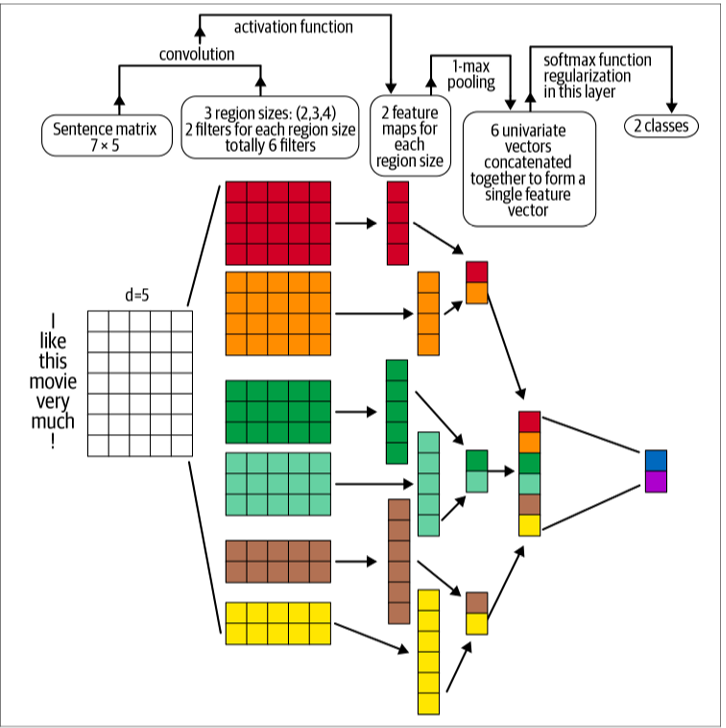
\includegraphics[width=0.8\textwidth]{imagenes/Cap 2/cnn.png}
	\caption{Diagrama de CNN}
	\label{fig:RNN}
	\cite{sowmya_practical_npl}
\end{figure}

\subsection{Tranformadores}

Los trasformadores son la ultima innovación en lo que respecta a modelos basados en DL para NLP.
Los
modelos de transformadores obtuvieron avances en la mayoría de las tareas de NLP en los últimos
años. \\
Estos modelan el contexto textual pero no de manera secuencial. Dada una palabra en una entrada de
texto, se
prefiere mirar las demás palabras vecinas en el texto y representar cada palabra de acuerdo a el
contexto
de las demás. Por ejemplo si el contexto habla de finanzas, entonces "banco" probablemente
representaría una
institución financiera. Por otro lado en el contexto de un rió, estaría relacionado con un
montículo de tierra.
Recientemente, los transformadores han sido utilizados para transferir aprendizaje con flujos de
pequeñas tareas,
La transferencia de aprendizaje es una técnica en IA en la cual lo que se aprendió en resolver un
problema es
aplicado para resolver problemas similares.

\begin{figure}[H]
	\centering
	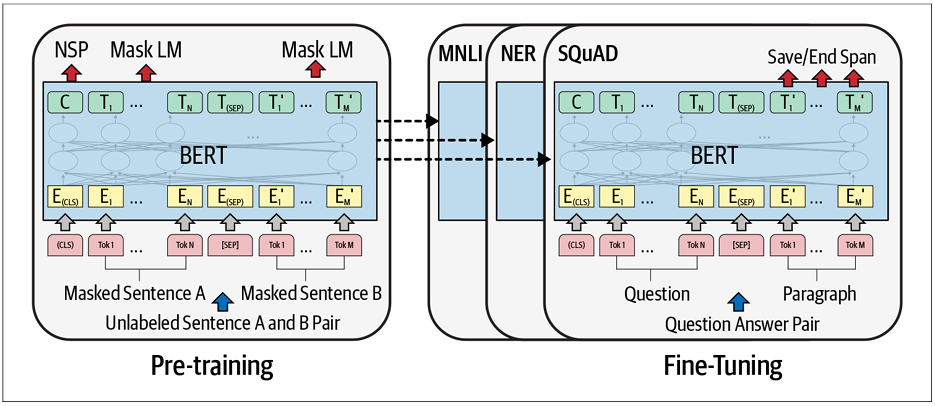
\includegraphics[width=0.8\textwidth]{imagenes/Cap 2/tranformers.png}
	\caption{Diagrama de un Transformador}
	\label{fig:RNN}
	\cite{sowmya_practical_npl}
\end{figure}

\subsection{Autoencoders}
Los autoencoders son otro tipo de red neuronal utilizadas principalmente para aprender a
representar la
entrada de forma comprimida en un vector. Por ejemplo, si queremos representar unas palabras en un
vector,
podemos aprender a mapear el texto en vectores y luego remapear para reconstruir la entrada
original.
Esto es una forma de aprendizaje no supervisado ya que no se necesitan datos anotados para el
entrenamiento.\\

\begin{figure}[H]
	\centering
	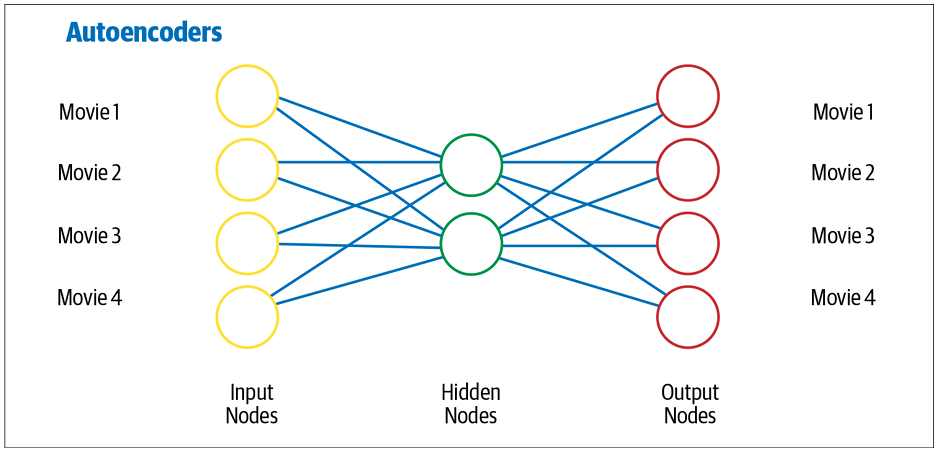
\includegraphics[width=0.8\textwidth]{imagenes/Cap 2/autoencoder.png}
	\caption{Representacion de un autoencoder}
	\label{fig:autoencoder}
	\cite{sowmya_practical_npl}
\end{figure}

%comparacion de metodos 

% TODO agregar aplicaciones 

\section{Chatbots}
% conceptos mas específicos
%---data adquisitcition

%----extraccion de texto

%----preprosesado

%----feature engineeniring 

%----modeling 

%---evaluation

%----post modelign 

\subsection{Concepto}
Los chatbots son programas que imitan la conversación humana utilizando la Inteligencia
Artificial.\cite{UniversityRelatedFAQS}
\subsection{Características}
Existen diferentes tipos de chatbots, clasificados según su complejidad, objetivos o funciones,
pero todos ellos cuentan con las siguientes cualidades según Nicol Radziwill y Morgan Benton
\cite{evaluating_quality}
\begin{itemize}
	\item Rendimiento: se refiere a la eficiencia en la asignación de funciones y a la robustez que
	      tienen en cuanto a la manipulación y a las entradas inesperadas.
	\item Funcionalidad: es capaz de interpretar, responder y ejecutar	correctamente las tareas
	      demandadas.
	\item Humanidad: la conversación con el chatbot debe ser natural, lo mas parecida a la humana.
	\item Ética: genera confianza, respeta y protege la dignidad, y la privacidad de los usuarios.
	\item Accesibilidad: se encuentra disponible cuando el usuario quiera usarlo, además se refiere
	      a que es capaz de detectar intenciones y significados
\end{itemize}
% documentación de rasa como referencia

\subsection{Aplicaciones}
Se pueden mencionar dos tipos de aplicaciones:
\begin{itemize}
	\item Asistentes Personales Virtuales: ofrecen servicios a los usuarios a través de texto o
	      voz. Ejemplos: Siri(Apple), Google Assistant, Alexa (Amazon) y Cortana (Microsoft)
	\item Bots para el consumo específico: sus aplicaciones son muy variadas, puede utilizarse en
	      el transporte, la salud, el clima, entretenimiento o incluso en la educación.
\end{itemize}
\subsection{Arquitectura}
Para el diseño adecuado de cualquier sistema la mejor solución es dividirla en varias partes o
subsistemas de acuerdo a un estándar.
En la figura \ref{fig:Arquitectura} se puede ver que existen dos bloques bien definidos, al primero
se lo llama 'lado del cliente' que es la parte que interactúa con los usuarios; y el segundo bloque
es el 'lado del servidor' encargado de procesar las peticiones del cliente.\\
\begin{figure}[h]
	\centering
	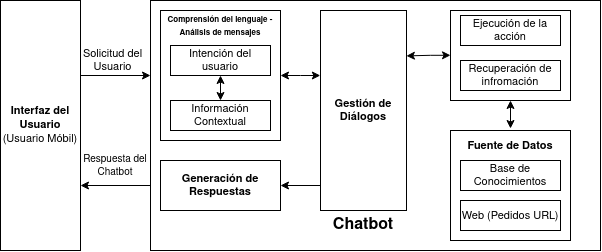
\includegraphics[width=\textwidth]{imagenes/Cap 2/Arquitectura.png}
	\caption{Arquitectura de los Chatbots}
	\label{fig:Arquitectura}
\end{figure}
\indent El  proceso inicia en la interfaz de usuario cuando el cliente realiza una solicitud, ésta
es analizada en el bloque componente de comprensión de lenguaje, aquí se extrae toda la información
necesaria y se deduce las intenciones del usuario.\\
\indent Una vez que el chatbot llegue a la mejor interpretación que puede, ejecuta las acciones
solicitadas o recupera la información de su fuente de datos, que puede ser una base de datos propia
o datos externos accedidos a través de APIs.\\
\indent Posteriormente se generan las respuestas lo más parecidas a las que daría una persona
humana, para ello utiliza la información de intención y contexto proveída por el componente de
análisis de mensajes del usuario.\\
\indent El componente de gestión de diálogo se encarga de solicitar información faltante,
aclaraciones y hacer preguntas de seguimiento.\cite{Overview_of_chatbots}

\subsection{Plataformas de desarrollo}
\begin{itemize}
	\item DialogFlow:
	      Es la plataforma de desarrollo de chatbots de Google, permite una fácil integración a
	      aplicaciones móviles y web, también facilita bastante el diseño de la interfaz de usuario.\\
	      Admite como entrada texto y voz, es capaz de responder a los clientes con texto o voz
	      sintética.\\
	      Existen dos versiones, Dialogflw CX utilizado para agentes grandes o muy avanzados y
	      Dialogflow ES que es la versión estándar, ésta cuenta con una versión gratuita.\\
	      El precio varia según la versión elegida y el tipo de entrada, Dialogflow ES cobra 0.002
	      USD por cada solicitud realizada por texto y 0.0065 USD si la entrada es un audio de hasta 15
	      segundos.\cite{Dialogflow}
	\item IBM Watson:
	      IBM Watson  permite a los usuarios integrar sus chatbots en cualquier canal, sea web,
	      aplicaciones o incluso una llamada.\\
	      Es capaz de aprender los vocabularios de la industria,	términos coloquiales o dialectos
	      regionales, admite entradas de voz y también de texto. \\
	      Está diseñada para aprender sobre el camino, proporciona herramientas para detectar las
	      tendencias y estas ayudan a asignar recursos de forma mas eficiente y eficaz.\\
	      No es necesario escribir ni una sola linea de código ya que utiliza un entorno de 'arrastre
	      y suelte' para construir los diálogos y una vez que lo adaptemos a nuestras necesidades, fácilmente
	      lo incorporamos a la app con 'copiar y pegar'.\cite{IBMCloud2020}\\
	      Cuenta con tres versiones: la versión mas básica, Lite, es gratuita pero muy limitada en
	      sus funcionalidades.
	      Luego vienen las versiones de paga, Plus y Enterprise con precios que van desde los 140 USD
	      por mes.\cite{IBM_Price}
	\item Amazon Lex:
	      Amazon Lex es la propuesta del gigante tecnológico Amazon, sirve para diseñar, crear,
	      probar e implementar interfaces de conversación en las aplicaciones.\\
	      Reconoce tanto entradas de texto como de voz, gestiona el contexto de las conversaciones de
	      forma nativa y también permite una gran fidelidad en las interacciones de habla telefónica.\\
	      La integración con plataformas se realiza de forma muy sencilla desde la consola de Amazon
	      Lex , permite aplicaciones web, móviles y los servicios propios de Amazon como Amazon Kendra,
	      Amazon Polly o AWS Lambda.\\
	      Los precios varían según el tipo de servicio solicitado, El mas básico 'Interacción de
	      respuesta y solicitud' cobra 0,004 USD por solicitud de voz y 0,00075 USD por solicitud de
	      texto.\cite{Amazon_Lex}
	\item RASA Open Source:
	      Es una plataforma de código abierto que proporciona procesamiento de lenguaje natural para
	      convertir los mensajes de los usuarios en intenciones y entidades que los chatbots entienden,
	      permite la gestión de los diálogos basándose en los mensajes de los usuarios y el contexto de la
	      conversación.\\
	      La integración a las aplicaciones mas comunes de mensajes y a los canales de voz se puede hacer
	      de forma muy sencilla con los conectores ya incorporados, para conectar a las demás aplicaciones
	      móviles o web se deben personalizar los conectores.\\
	      RASA también tiene una versión de paga denominada RASA Enterprise, utilizada para el despliegue
	      a escala, su precio varía de acuerdo a las necesidades de la organización y del
	      proyecto.\cite{Rasa}
	\item Chatterbot:
	      Chatterbot es una librería de Python que facilita la automatización de respuestas mediante
	      distintos algoritmos de aprendizaje automático, esto permite que una instancia de agente mejore su
	      propio conocimiento de las posibles respuestas a medida que interactúa con humanos y otras fuentes
	      de datos informativos\\
	      Cada vez que un usuario introduce una frase, la librería guarda el texto que ha introducido y
	      el texto al que responde la frase. A medida que ChatterBot recibe más entradas, aumenta el número
	      de respuestas que puede dar y la precisión de cada respuesta en relación con la declaración
	      introducida.\\
	      Se puede integrar a las aplicaciones mediante APIs, además ChatterBot tiene soporte directo
	      para la integración con el ORM de Django, esto facilita bastante para crear las páginas
	      conversacionales.\cite{Chatterbot}\\
\end{itemize}

\indent Haciendo una comparación entre todas las herramientas analizadas, vemos que la creación de
los chatbots con Dialogflow, IBM Watson y Amazon Lex es mucho mas sencilla, ya que tienen una
madurez tecnológica muy alta, gran soporte y las interfaces son muy intuitivas, además no requieren
de mucha programación. La mayor desventaja es que las versiones que cuentan con todas las
funcionalidades son de paga, y las versiones gratuitas son muy limitadas y básicas, por lo que
descartamos estas tres opciones.\\
\indent En cuanto a Chatterbot y RASA, la curva de aprendizaje puede ser un poco mayor porque no
utilizan interfaces gráficas, todo es programado con Python, un lenguaje muy versátil que cuenta
con numerosas librerias, esto permite tener mayor control sobre los chatbots porque se pueden
manipular todos los ficheros y modificar las configuraciones, Si bien ambos están muy bien
documentados, RASA destaca de Chatterbot por su comunidad, cuenta incluso con un foro donde
participan los desarrolladores y usuarios dispuestos a brindar ayuda a todo aquel que las
necesite.\\
\indent Teniendo en cuenta que no contamos con experiencia en el desarrollo de chatbots, se valora
de sobremanera la comunidad, documentación y tutoriales con los que cuenta RASA, además que permite
la integración con distintas plataformas y el lenguaje de programación que utiliza (Python) es de
nuestro conocimiento, es por eso que concluimos con que RASA es una buena elección para llevar a
cabo este proyecto.
    
\chapter[RASA]{RASA Open Source}
Rasa es un framework que permite la construcción de forma sencilla de chatbots personalizados, está compuesta de dos librerias de código abierto, Rasa NLU y Rasa Core, denominadas en conjunto Rasa Stack.
\indent 
\section{Conceptos Básicos}
\begin{itemize}
    \item \textbf{intents (intenciones): }son las categorías, denominadas utterances creadas para lo que el usuario está tratando de transmitir o lograr en una conversación, por ejemplo 'saludos' donde se especifican las distintas formas de saludar. Las intenciones pueden ser divididas en pequeñas subintenciones denominadas 'Retrieval Intent'.
    \item \textbf{entities (entidades): } las entidades son informaciones o palabras clave que pueden ser extraídas de un mensaje para personalizar la conversación.
    \item \textbf{slots:} es un registro de datos que Rasa utiliza para guardar la información proveída por el usuario en el curso de la conversación, un claro ejemplo del uso de este elemento es almacenar el nombre del usuario para personalizar los mensajes.
    \item \textbf{responses (respuestas):} mensajes que los chatbots envían a los usuarios, estos pueden ser dinámicos y con cualquier tipo de contenido como texto, imágenes, links, etc.
    \item \textbf{forms (formularios):} Un tipo de acción personalizada que pide al usuario varios datos.
    \item \textbf{actions (acciones):} es un paso que toma el bot en la conversación por ejemplo, llamar a una API o enviar una respuesta al usuario.\cite{Glossary}
\end{itemize}

\section{Cómo se lleva a cabo las conversaciones?}
Para llevar a cabo las conversaciones se utilizan las dos librerías del Rasa Stack.
\begin{itemize}
    \item \textbf{Rasa NLU: } En ella  se escriben los archivos de configuración, se elige el pipeline y el modelo de entrenamiento para que deduzca las intenciones y posteriormente pueda extraer las entidades disponibles.\\
    \indent Puede ser basado en reglas o en redes neuronales, el primero suele ser mas ligero y no necesita de muchos datos aunque no son buenos en tareas antes no vistas, mientras que el segundo necesita de mas capacidad de cómputo y datos para entrenamiento, son mas flexibles que los basados en reglas, ya que pueden aprender cosas que no han visto antes.
    \item \textbf{Rasa Core: } es el gestor de diálogos utilizado para crear modelos que sean capaces de decidir que respuestas o acciones se ejecutarán de acuerdo a las entradas generadas por el usuario.\\
    \indent También puede ser basado en reglas, que es el enfoque mas tradicional, funciona muy bien en muchos casos pero es difícil de expandir las conversaciones, también puede ser basado en redes neuronales que escoge la siguiente acción basándose en la conversación y en los ejemplos del entrenamiento.
\end{itemize}
\indent Básicamente, Rasa NLU se encarga de interpretar los mensajes y Rasa Core de de decidir que acción tomar.\\
\indent Para asegurarnos de que una conversación funcione Rasa utiliza un proceso denominado ‘conversation-driven development’ que consiste en revisar manualmente las conversaciones para detectar cualquier error cometido, agregar nuevos datos de entrenamiento, volver a entrenar el modelo y probarlo nuevamente\cite{Introduction_to_Rasa}
\section[Instalación de RASA]{Instalación}
Primeramente crearemos un entorno virtual denominado 'venv' utilizando Python en una computadora con Linux.

\begin{center}
    \framebox[10cm][c]{python3 -m venv ./venv}  
\end{center}
Luego se activa el entorno virtual.
\begin{center}
    \framebox[10cm][c]{source ./venv/bin/activate}   
\end{center}
Y por último se instala Rasa Open Source utilizando pip (requiere Python 3.7 o 3.8)
\begin{center}
    \framebox[10cm][c]{sudo pip3 install -U –user pip \&\& pip3 install rasa}    
\end{center}

\section{Creación de un Proyecto}
\indent La creación de un nuevo proyecto se realiza con el comando 'rasa init', éste crea un conjunto de carpetas y archivos así como se muestra en la figura \ref{fig:Estructura}.
\begin{figure}[h]
    \centering
    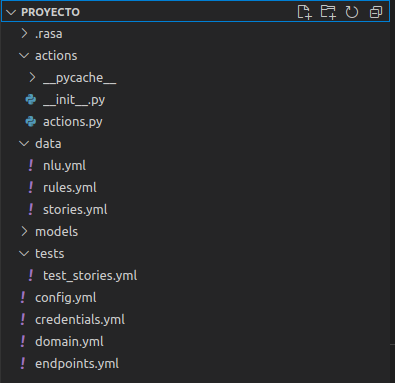
\includegraphics[width=\textwidth]{imagenes/cap3/4_Estructura del Proyecto.png}
    \caption{Estrucutra de los archivos}
    \label{fig:Estructura}
\end{figure}
\subsection{Archivo nlu}
En él se encuentran datos estructurados que sirven para entrenar el modelo y luego extraer la información de los mensajes del usuario. Estos datos son  las intenciones y entidades, también se pueden agregar expresiones regulares y algunas tablas de búsqueda. \cite{NLU_Documentation}

\subsection{Archivo Rules}
En este archivo se definen las reglas, que no son mas que  tipo de datos de entrenamiento encargados de describir partes de una conversación que siempre sigue el mismo camino.\cite{Rules_Documentation}

\subsection{Archivo Stories}
Las historias son un tipo de datos de entrenamiento, se utiliza para entrenar modelos que puedan generalizar las rutas de conversación. Las entradas del usuario son expresadas mediante intents, y entitites si es necesario,  mientras que las respuestas del asistente son expresadas mediante actions.\\
Los patrones que siguen las conversaciones podemos extraer de datos ya existentes o con la herramienta de rasa 'interactive learning'.\cite{Stories_Documentation}

\subsection{Archivo config}
En el archivo config se definen el lenguaje y los componentes del pipeline, que forman parte de Rasa NLU y las políticas a ser utilizadas, correspondiente a Rasa NLU.\\
El pipeline es el encargado de definir la dirección de flujo de datos entre los diferentes componentes, Rasa nos permite configurar cada uno de ellos según nuestras necesidades, de tal forma que podamos realizar las predicciones de las intenciones y la extracción de las entidades. Las políticas forman parte de la gestión de diálogos, encargada de seleccionar la siguiente acción a ser ejecutada.\cite{Configuration_Documentation}\\
La configuración del pipeline y las políticas son de suma importancia, por lo que se detallaran sus componentes en la sección \ref{ch:Componentes}.

\subsection{Archivo credentials}
Aquí se definen los credenciales para las plataformas de voz y chat que el bot utiliza. Rasa cuenta con algunos conectores preestablecidos para los canales mas conocidos como Facebook Messenger, Telegram, Google Hangouts Chat o una pagina web propia.\cite{Credentials_Documentation}

\subsection{Archivo domain}
El archivo domain es un archivo de configuración donde se especifican las intenciones, entidades, slots, respuestas, formularios y acciones que el bot debe saber.\cite{Domain_Documentation}

\subsection{Archivo endpoints}
Los endpoints son los enlaces a los servicios externos o internos que puede tener Rasa. En el se definen los servidores que corren o en los que están alojadas las acciones personalizadas, al igual que los modelos con los que se cuenta. También es aquí donde se especifican los tracker store, utilizados para guardar las conversaciones, y los event broker, encargados de conectar el bot con otros servicios que procesan los datos que llegan de las conversaciones.

\section{Componentes}\label{ch:Componentes}
% de https://rasa.com/blog/intents-entities-understanding-the-rasa-nlu-pipeline/
En esta sección estaremos describiendo el funcionamiento de los componentes utilizados en la arquitectura de Rasa, 
estos componentes son modulares y genéricos para lo que son sistemas de NLU modernos, pueden ser propios del
entorno o proveídos por otras librerías de terceros para extender funcionalidades.

\begin{figure}[h]
    \centering
    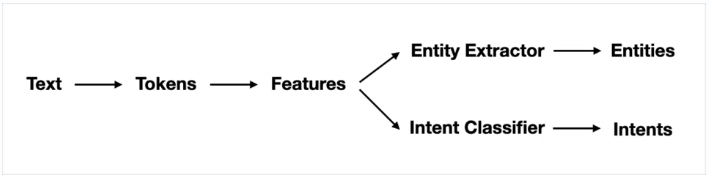
\includegraphics[width=\textwidth]{imagenes/cap3/rasa_components.png}   
    \caption{Componentes de un esquema NLU}
    \label{fig:Componentes-MLU}
\end{figure}

\subsection{Tokenizadores}
Antes de poder ser procesada una porción de texto debe ser dividida en porciones mas pequeñas, para esto se suele utilizar 
un tokenizador (o tokenizer).   Este divide el texto en componentes de un vector.\\ Algunos tokenizadores también
agregan información extra a los tokens que pueden ser usados para generar lemas, o sea extraer la palabra que da el significado base a las palabras que pueden ser utilizados por el contador de vectores.\\
Para el Inglés y el Español usualmente se usa WhiteSpaceTokenizer que separa en tokens cuando se detectan espacios, para los idiomas que no precisen de espacios en blanco para separar las palabras como el Coreano, Japones o Chino, se utilizan MitieTokenizer, en el caso del último tambien es muy frecuente el uso de JiebaTokenizer.\cite{warmerdam_2022}

\begin{figure}[h]
    \centering
    
\includegraphics[width=\textwidth]{imagenes/cap3/tokenization.png}   
    \caption{Tokenización}
    \label{fig:tokenization-MLU}
\end{figure}

\subsection{Caracterizadores}
 Los caracterizadores generan pesos numéricos para ser consumidos por los modelos de ML. Existen dos tipos principales de
 características, las Dispersas(Sparse Features) que usualmente cuentan lo que pueden representar subpalabras o características
 léxicas y las Densas(Dense Features) estos suelen consistir en porciones preentrenadas, para que
 estos se desempeñen correctamente se debe seleccionar un Tokenizador apropiado. \cite{warmerdam_2022}
 Todos los caracterizadores son presentados en la tabla \ref{tab:Caracterizadores}

\begin{table}[]
\resizebox{\textwidth}{!}{%
\begin{tabular}{|l|l|l|}
\hline
\textbf{Caracterizador}    & \textbf{Requisitos}     & \textbf{Tipo}                                                                  \\ \hline
MitieFeaturizer            & MitieNLP                & Dense featurizer                                                               \\ \hline
SpacyFeaturizer            & Dense / Sparse Features & \begin{tabular}[c]{@{}l@{}}Logistic Regression de \\ scikit-learn\end{tabular} \\ \hline
ConveRTFeaturizer          & Tokenization            & Dense featurizer                                                               \\ \hline
LanguageModelFeaturizer    & Tokenization            & Dense featurizer                                                               \\ \hline
CountVectorsFeaturizer     & Tokenization            & Sparse featurizer                                                              \\ \hline
LexicalSyntactitFeaturizer & Tokenization            & Sparse featurizer                                                              \\ \hline
RegexFeaturizer            & Tokenization            & Sparse featurizer                                                              \\ \hline
\end{tabular}%
}
    \caption{ Caracterizadores. Elaboración Propia}
    \label{tab:Caracterizadores}
\end{table}

\begin{figure}[h!]
    \centering
    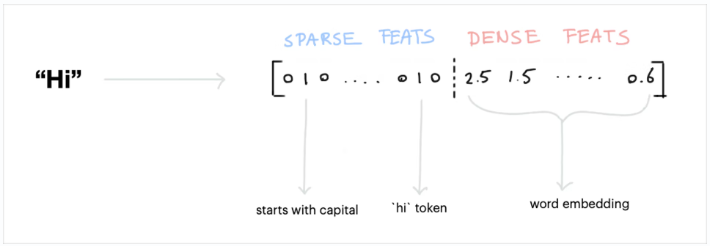
\includegraphics[width=\textwidth]{imagenes/cap3/featurizers.png}   
    \caption{Caracterización}
    \label{fig:feazturization-MLU}
\end{figure}

\subsection{Clasificadores de Intención(Intent Classiffiers)}

Una vez que se generaron las características para todos los tokens y para toda la oración, podemos pasarlos a un
modelo clasificador de intenciones. Rasa por defecto usa el modelo DIET que puede encargarse tanto de 
la clasificación de la intención y extracción de entidades. También puede aprender tanto de características de Tokens como de oraciones. \cite{warmerdam_2022}
% Please add the following required packages to your document preamble:
% \usepackage{graphicx}
\begin{table}[]
\resizebox{\textwidth}{!}{%
\begin{tabular}{|l|l|l|}
\hline
\textbf{Clasificador}        & \textbf{Requisitos}     & \textbf{Utiliza}                                                                              \\ \hline
MitieIntentClassifier        & MitieNLP                & Clasificación multiclase con SVM                                                              \\ \hline
LogisticRegressionClassifier & Dense / Sparse Features & Logistic Regression de scikit-learn                                                           \\ \hline
SklearnIntentClassifier      & Dense Features          & \begin{tabular}[c]{@{}l@{}}SVM lineal optimizado con búsqueda \\ en cuadrícula\end{tabular}   \\ \hline
KeywordIntentClassifier      & Ninguno                 & Comparador de palabras clave                                                                  \\ \hline
DIETClassifier               & Dense Features          & Transformadores                                                                               \\ \hline
FallbackClassifier           & Intents                 & \begin{tabular}[c]{@{}l@{}}Requiere de un clasificador de \\ intenciones previo\end{tabular} \\ \hline
\end{tabular}%
}

\caption{Clasificadores de intenciones. Elaboracion propia}
\label{IntentClassifier}
\end{table}
\begin{figure}[h]
    \centering
    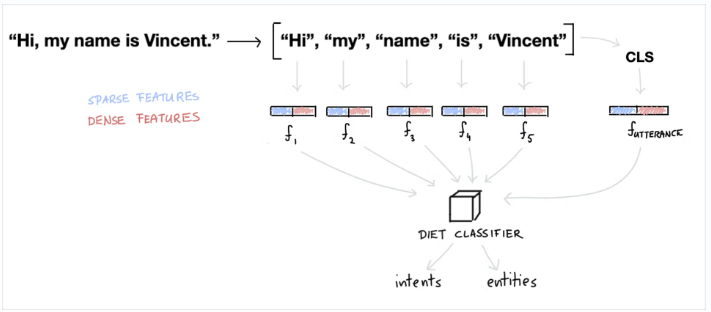
\includegraphics[width=\textwidth]{imagenes/cap3/intent_classiffier.png}   
    \caption{Clasificación de intenciones y entidades}
    \label{fig:intentclasification-MLU}
\end{figure}



\subsection{Extracción de entidades}

Además de DIET, existen otros clasificadores basados en ML que pueden aprender como detectar entidades, estos no son recomendados para todos los casos, también puede ser implementado un extractor basado en Expresiones
Regulares(RegexEntityExtractor) \cite{warmerdam_2022}
% Please add the following required packages to your document preamble:
% \usepackage{graphicx}

\begin{table}[h!]
\resizebox{\textwidth}{!}{%
\begin{tabular}{|l|l|l|}
\hline
\textbf{Clasificador}   & \textbf{Requisitos} & \textbf{Utiliza}                                                            \\ \hline
MitieEntityExtractor    & MitieNLP            & \begin{tabular}[c]{@{}l@{}}Clasificación multiclase \\ con SVM\end{tabular} \\ \hline
SpacyEntityExtractor    & SpacyNLP            & Modelo estadístico BILOU                                                    \\ \hline
CRFEntityExtractor      & Tokens              & Campo aleatorio condicional (CRF)                                           \\ \hline
DucklingEntityExtractor & Ninguno             & Expresiones regulares                                                       \\ \hline
DIETClassifier          & Dense Features      & Transformadores                                                             \\ \hline
RegexEntityExtractor    & Ninguno             & Tablas de búsqueda                                                          \\ \hline
\end{tabular}%
}
\caption{Extractores de entidades. Elaboración propia}
\label{EntityExtractor}
\end{table}
\begin{figure}[h]
    \centering
    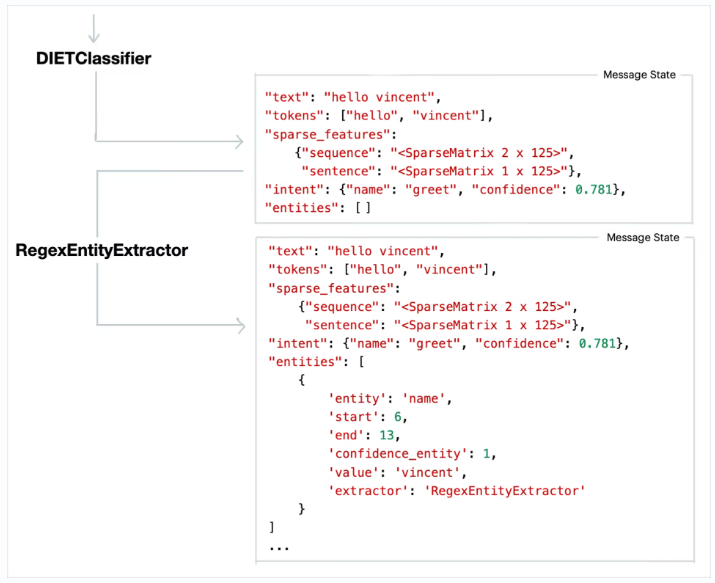
\includegraphics[width=\textwidth]{imagenes/cap3/regex_extractor.png}   
    \caption{Extractor Regex}
    \label{fig:regex-extractor}
\end{figure}

\subsection{Selectores}
Los selectores se encargan de predecir la respuesta de un conjunto de respuestas posibles para los retrieval intents, son utilizados posteriormente por el gestor de diálogo para dar la respuesta mas adecuada.
Utiliza la misma arquitectura y optimización que el DIETClassifier.


\subsection{Predicción de acciones}
\begin{figure}[h!]
    \centering
    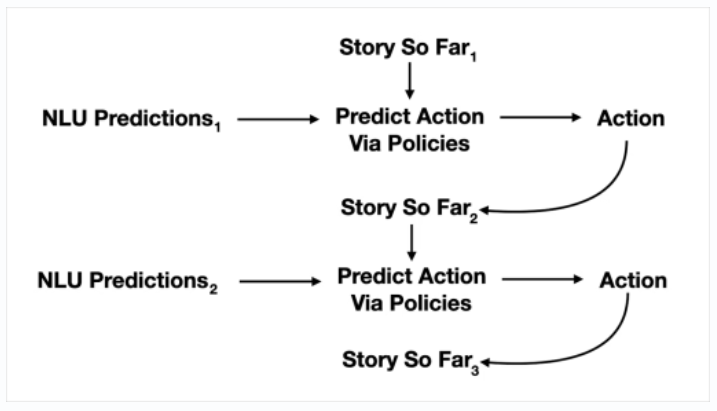
\includegraphics[width=\textwidth]{imagenes/cap3/predicciones.png}   
    \caption{Predicción de acciones.}
    \label{fig:regex-extractor}
\end{figure}

Con el flujo NLU, se detectan las entidades e intenciones. Pero este flujo no predice la siguiente acción en la 
conversación. Para esto se utiliza el flujo de política. Las políticas aseguran el uso de predicciones de NLU así como 
también el estado presente de la conversaciones para decidir que acción tomar, pueden ser basado en reglas o en aprendizaje automático.\\
\textbf{Políticas basadas en Aprendizaje Automático:}
\begin{itemize}
    \item \textbf{TED Policy:}
    Es un conjunto de algoritmos desarrollados por RASA para la predicción de diálogo y reconocimiento de entidades. Su arquitectura se basa en transformadores que convierten el diálogo actual en un vector de diálogos, para compararlos con otros vectores en busca del mas cercano, a partir de las acciones existentes.\cite{ConversationalAIwithRasa}
    \item \textbf{UnexpecTED Intent Policy:} Es una política auxiliar, tiene la misma arquitectura que TEDPolicy pero éste aprende cuales son las intenciones mas probables a ser expresadas según el contexto de la conversación. Siempre debe usarse en conjunto con al menos una otra política.\cite{UnexpecTED}
    \item \textbf{Memoization Policy: }Esta política utiliza las historias y acciones de los datos de entrenamiento y las guarda en un diccionario, si la conversación actual no coincide con ningun ejemplo, predice un 0.0.\cite{MemoizationPolicy}
    \item \textbf{Augmented Memoization Policy: } Tiene las mismas funcionalidades de Memoization Policy, pero además cuenta con un mecanismo que permite olvidar de forma aleatoria algunas partes de la conversación, luego predice las acciones ya con la historia reducida.\cite{AugmentedMemoizationPolicy}
\end{itemize}
\textbf{Políticas basadas en Reglas:}
\begin{itemize}
    \item \textbf{Rule Policy:} Realiza las predicciones basandose en reglas que se tienen en los datos de entramiento.
\end{itemize}
Con cada interacción, las políticas definidas indican con un nivel de confianza cuál será la siguiente acción a ser tomada, aquella que tiene obtiene el mayor resultado sera la que decida la siguiente acción, en caso de que se prediga con la misma confianza, se tiene en cuenta la siguiente asignación de importancia.
\begin{itemize}
    \item 6 - RulePolicy
    \item 3 - MemoizationPolicy o AugmentedMemoizationPolicy
    \item 2 -  UnexpecTEDIntentPolicy
    \item 1 - TEDPolicy
\end{itemize}

\section{Patrones de Conversación}
\subsection{Chitchat y FAQs}
Las preguntas frecuentes y los chitchats (conversaciones sobre temas no importantes) son casos donde el asistente siempre tiene que responder de la misma forma, sin importar el contexto de la conversación. El problema se encuentra en que si creamos intenciones y acciones para cada pregunta que se realiza, las historias y reglas serán muy extensas, es por eso que estas preguntas frecuentes las agrupamos en una 'retrieval intent' y se selecciona la respuesta correcta mediante el componente 'Response Selector'.\\
Para poder utilizarlo se debe configurar apropiadamente el archivo config.yml. Este componente utiliza la política basada en reglas 'RulePolicy', también caracterizadores y clasificadores de intenciones por lo que debe ubicarse en el pipeline después de estos.
\subsection{Fallbacks}
Para los casos donde el usuario pregunta algo que está fuera del alcance del bot, establecemos una intención llamada 'out of scope' a la que asociamos a una respuesta genérica y creamos una regla en el archivo rules.yml.\\ Existen casos donde la confianza en la clasificación es muy baja, esto implica que no se pueda predecir con buena confianza si se trata de una intención 'out of scope', para ello Rasa tiene una opción llamada 'Fallback' que permite pedir al usuario que reformule su pregunta para tratar nuevamente de predecir correctamente a que intención se refiere. \\
Para su utilización se debe agregar el 'FallbackClassifier' en el pipeline, crear respuestas por defecto y actualizar las reglas.
\section{Pruebas}
Rasa cuenta con varias funciones para probar los diálogos, historias, el gestor de diálogos y el procesamiento de mensajes.
\subsection{Validación de datos}
El comando 'rasa data validate' se encarga de verificar que no haya errores e inconsistencias en los datos y configuraciones. Es recomendable ejecutar este comando antes de entrenar el modelo, ya que si se encuentra algún problema, el entrenamiento también podría fallar.
\subsection{Evaluación del desempeño de la NLU}
Una practica usual al ejecutar aprendizaje automático es dividir aleatoriamente el conjunto de datos en uno de entrenamiento y otro de pruebas. El bot utiliza el primer conjunto para aprender las características necesarias para realizar las predicciones adecuadas, y el segundo conjunto para evaluar el modelo mediante datos que aún no hayan sido vistos antes.\\
Rasa nos permite dividir los datos mediante el comando 'rasa data split nlu' que por defecto separa los datos de entrenamiento/prueba en un 80/20, luego, para probar que tan bien entrenado se encuentra el modelo utilizamos 'rasa test nlu' especificando cuales son los datos de entrenamiento y prueba de la siguiente forma:\\
    --nlu train\_test\_split/test\_data.yml

Otro método muy completo para evaluar el modelo es mediante validación cruzada o cross validation. Este divide los datos en múltiples subconjuntos llamados 'folds' donde se van alternando los datos de entrenamiento y pruebas

\section{Despliegue del sistema}
Según la documentación de Rasa, el mejor momento para desplegar una versión de prueba es tan rápido cuando 
se tenga un bot que cumpla los requisitos mínimos de los requisitos de diseño. De esta manera se puede
tener pruebas de usuarios reales lo mas rápido posible y poder agregar estos casos.

\subsection{Arquitectura}

\begin{figure}[h]
    \centering
    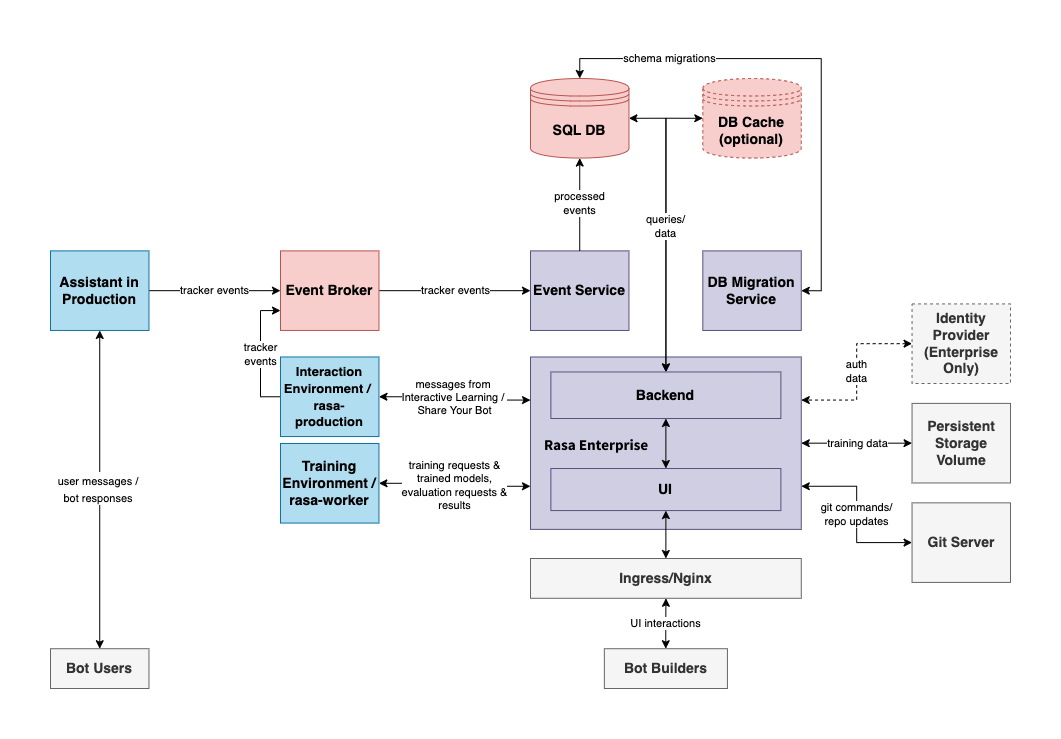
\includegraphics[width=\textwidth]{imagenes/cap3/architecture_deploy.png}   
    \caption{Arquitectura}
    \label{fig:deploy-architecture}
\end{figure}

\subsubsection{Servicios}
El diagrama muestra tres categorías de servicios: Los morados son componentes de principales de Rasa
Enterprise, los azules son los servicios principales de Rasa Open Source y los anaranjados son servicios 
de terceros.

Tanto los componentes de Rasa Open Source e Enterprise tienen bases de datos independientes. Los eventos
datos de conversaciones fluyen desde los servicios de Rasa Open Source a Rasa Enterprise a través del event broker.

\subsubsection{Servicios de Rasa Enterprise}

Los servicios de Rasa Enterprise, no son todos de libre uso, algunas partes se utilizan bajo un modelo de 
licencias. Pero estos si bien no son indispensables (pueden ser reemplazados por servicios libres de terceros) hacen que el despliegue de el producto sea mucho mas sencillo y así como también su desarrollo. Dicho esto pasamos a explicar los existentes en el diagrama, se tratan de los 3 mínimos servicios para 
ejecutar Rasa Enterprise estos deben ser todos de la misma versión para asegurar compatibilidad. 

\begin{itemize}
     \item \textbf{Servicio de eventos(Event Service):} Consume datos del corredor de eventos(event 
    broker) y los archiva en la base de datos.
     \item \textbf{Servicio de migración de la Base de datos(DB migration service):}  Asegura que los esquemas de la base de datos
     esten actualizados con respecto a la versión actual de Rasa Enterprise.
    \item \textbf{Rasa-X:} Ejecuta las tareas del back-end y front-end. Archiva y recupera datos de 
    conversaciones, entrenamiento y meta-datos, como rótulos de conversaciones y banderas de mensajes
    en la base de datos de Rasa Enterprise. El front-end usa las entradas del back-end para brindar una 
    interfaz amigable para el usuario.
\end{itemize}

\subsubsection{Servicios de Rasa Open Source}

Los servicios de Rasa Open Source se ejecutan de manera totalmente independiente de Rasa Enterprise, 
por otro lado Rasa Enterprise si depende de Rasa Open Source para manejar los datos de las conversaciones,
entrenamiento y ejecución de modelos. En orden para que Rasa Enterprise pueda mostrar conversaciones
tomadas por Rasa Open Source este publica los eventos de una conversación a el mismo event broker
al cual Rasa Enterprise esta consumiendo.

\subsubsection{Partes}

\begin{itemize}
     \item \textbf{rasa-production:} Es el servicio que ejecuta el modelo entrenado, usado para 
     parsear mensajes en intents y predecir acciones en conversaciones con el usuario, en un canal o 
     en UI de Rasa Enterprise.
     \item \textbf{rasa-worker:} Es utilizado para servicios de segundo planos, como para entrenar un
     nuevo modelo.
    \item \textbf{app:} Es el servidor de acciones personalizadas, ejecutan acciones especificas
    de la aplicación.
\end{itemize}
\chapter[IMPLEMENTACION]{IMPLEMENTACIÓN}
En el capitulo anterior, un diagrama de bloques de una arquitectura recomendada.Puesto a que nuestra implementación que para una cantidad limitada de usuarios  y como asi también para no depender de componenetes propietarios o
de pago  realizamos algunos cambios a esta arquitectura a probechando la interoperavilidad de Rasa Open Source. 

\begin{figure}[h]
    \centering
    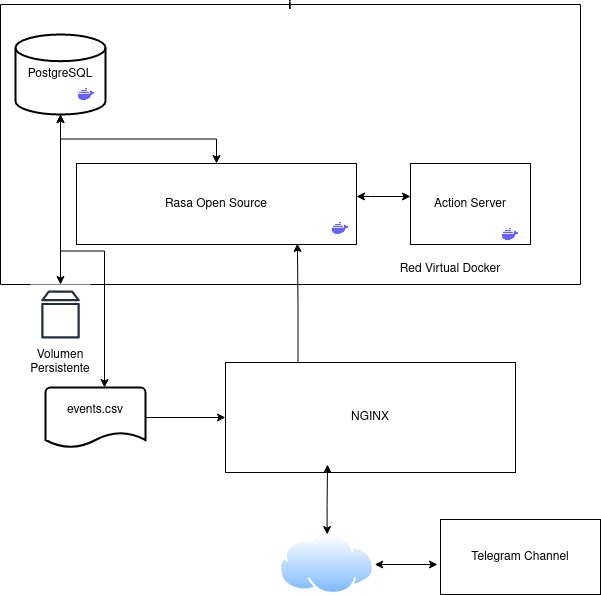
\includegraphics[width=\textwidth]{imagenes/cap4/server.png}
    \caption{Implementación Final}
    \label{fig:server_diagram}
\end{figure}



\chapter[ANÁLISIS]{ANÁLISIS DE RESULTADOS}
En este capítulo se presentan los resultados obtenidos en la implementación del chatbot utilizando
la plataforma Rasa OpenSource para responder preguntas frecuentes de estudiantes de la Facultad de
Ingeniería.  Además, se analizan los datos recopilados durante el entrenamiento del modelo, se
discuten las limitaciones, evaluara la efectividad del chatbot, asi como tambien posibles mejoras
en la implementación del chatbot.

\section{Configuraciones ulilizadas}
Dado el interés en que los resultados obtenidos sean replicables, en primer lugar, se explicarán
los componentes seleccionados para el entrenamiento y despliegue del modelo.
\begin{itemize}
	\item \textbf{WhitespaceTokenizer}: componente que divide el texto en palabras
	      individuales, utilizando espacios en blanco como delimitador.
	      \cite{Configuration_Documentation}
	\item \textbf{RegexFeaturizer}: componente que crea características basadas en expresiones
	      regulares. Esto puede ser útil para detectar patrones en el texto.
	      \cite{Configuration_Documentation}
	\item \textbf{LexicalSyntacticFeaturizer}: componente que combina características léxicas y
	      sintácticas para crear una mejor representación del texto. Utiliza etiquetas de
	      partes del discurso
	      y etiquetas de análisis de dependencia para crear características.
	      \cite{Configuration_Documentation}
	\item \textbf{CountVectorsFeaturizer}: componente que crea una representación dispersa de
	      bolsa de
	      palabras del texto. Puede ser utilizado para crear características para la
	      clasificación de
	      intenciones o la extracción de entidades. \cite{Configuration_Documentation}
	\item \textbf{DIETClassifier}: componente que combina una red neuronal recurrente con un
	      transformador para realizar la clasificación de intenciones y el reconocimiento de
	      entidades.
	      Utiliza múltiples fuentes de información, como incrustaciones de palabras,
	      incrustaciones de
	      caracteres y etiquetas de partes del discurso. \cite{Configuration_Documentation}
	\item \textbf{EntitySynonymMapper}: componente que mapea las entidades a su forma canónica.
	      Esto
	      puede ser útil para manejar variaciones en la forma en que se expresan las entidades
	      en el texto. \cite{Configuration_Documentation}
	\item \textbf{ResponseSelector}: componente que selecciona una respuesta basada en la
	      entrada del
	      usuario. Utiliza un enfoque basado en recuperación, donde coincide la entrada del
	      usuario con un
	      conjunto de respuestas predefinidas. Puede ser útil para manejar preguntas frecuentes
	      o
	      conversaciones informales.\cite{Configuration_Documentation}
	\item \textbf{FallbackClassifier}: componente que clasifica los mensajes como fallback si
	      no
	      coinciden con ninguna de las intenciones en el modelo. Puede ser útil para manejar
	      mensajes fuera
	      de contexto o solicitudes que el modelo no está entrenado para
	      manejar.\cite{Configuration_Documentation}
\end{itemize}
\section{Conjunto de Datos propio}

Inicialmente, se creó un conjunto de datos con las posibles preguntas frecuentes de los alumnos,
una vez que el Bot estuvo en funcionamiento e integrado a Telegram se recolectaron las preguntas
que realmente tienen los estudiantes de la FIUNA, estas fueron guardadas en una base de datos como
eventos, teniendo mucha información innecesaria para el conjunto de datos. Para un mejor manejo y
limpieza de los datos se utilizó Python con ayuda de la librería Pandas. Posteriormente se guardó
el dataframe creado en un archivo de Excel donde se analizaron y clasificaron un total de 1051
entradas en 141 intenciones distintas, De entre ellas, se identificaron las 15 intenciones más
recurrentes.

\begin{figure}[H]
	\centering
	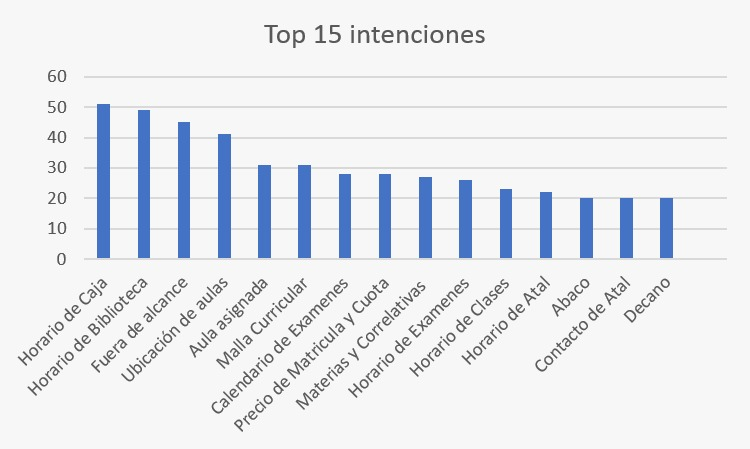
\includegraphics[width=\textwidth]{imagenes/cap5/Top15intents.jpeg}
	\caption{Top 15 Intenciones}
	\label{fig:Top15intents}
\end{figure}

\section{Validación de los datos e Historias}
Rasa cuenta con varias funciones para probar los diálogos, historias, gestor de diálogos y el
procesamiento de mensajes, de tal forma a encontrar errores o inconsistencias antes de realizar el
entrenamiento.

\subsection{Validación de datos}
El siguiente comando se encarga de verificar que no haya errores e inconsistencias en los datos y
configuraciones.

\begin{center}
	\framebox[10cm][c]{rasa data validate}
\end{center}

Es recomendable ejecutarlo antes de entrenar el modelo, ya que si se encuentra algún problema, el
entrenamiento también podría fallar.

\subsection{Evaluación del desempeño de la NLU}
Una práctica usual al ejecutar aprendizaje automático es dividir aleatoriamente el conjunto de
datos en uno de entrenamiento y otro de pruebas. El bot utiliza el primer conjunto para aprender
las características necesarias para realizar las predicciones adecuadas, y el segundo conjunto para
evaluar el modelo mediante datos que aún no hayan sido vistos antes.\\
Rasa nos permite dividir los datos mediante el comando:

\begin{center}
	\framebox[10cm][c]{rasa data split nlu}
\end{center}

Por defecto, Rasa separa los datos de entrenamiento/prueba en un 80/20, luego, para probar que tan
bien entrenado se encuentra el modelo utilizamos 'rasa test nlu' especificando cuales son los datos
de entrenamiento y prueba de la siguiente forma:\\

\begin{center}
	\framebox[10cm][c]{    --nlu train\_test\_split/test\_data.yml}
\end{center}

Rasa test proporciona herramientas que facilitan la detección y corrección de errores, incluye una
matriz de confusión, un archivo .json de reporte, un histograma de confianza y un archivo .json de
errores en caso de que existan.\\
La matriz de confusión es una herramienta fundamental que permite evaluar el rendimiento de un
modelo, permite identificar los falsos positivos y falsos negativos, nos muestra en su eje vertical
las etiquetas reales y en el eje horizontal las etiquetas predecidas, permitiendo identificar si
existen errores de clasificación.\\
Además, el script de rasa test guarda estos errores de clasificación en un archivo .json lo que
facilita el depurado y corrección de errores para mejorar la calidad de la clasificación.\\
El Histograma nos permite visualizar las predicciones del modelo y la confianza que ha sido
otorgada a cada intención o entidad.\\
Las predicciones correctas se encuentran en la parte izquierda del gráfico y son representadas en
color azul, mientras que las incorrectas se encuentran a la derecha y son de color rojo.\\
La ubicación de cada predicción en el eje horizontal del histograma representa el número de
muestras, y en el eje vertical la confianza con la que el modelo ha realizado su
predicción. \cite{interpretacion_graficos}

\subsection{Clasificador de Intenciones}

\begin{figure}[H]
	\centering
	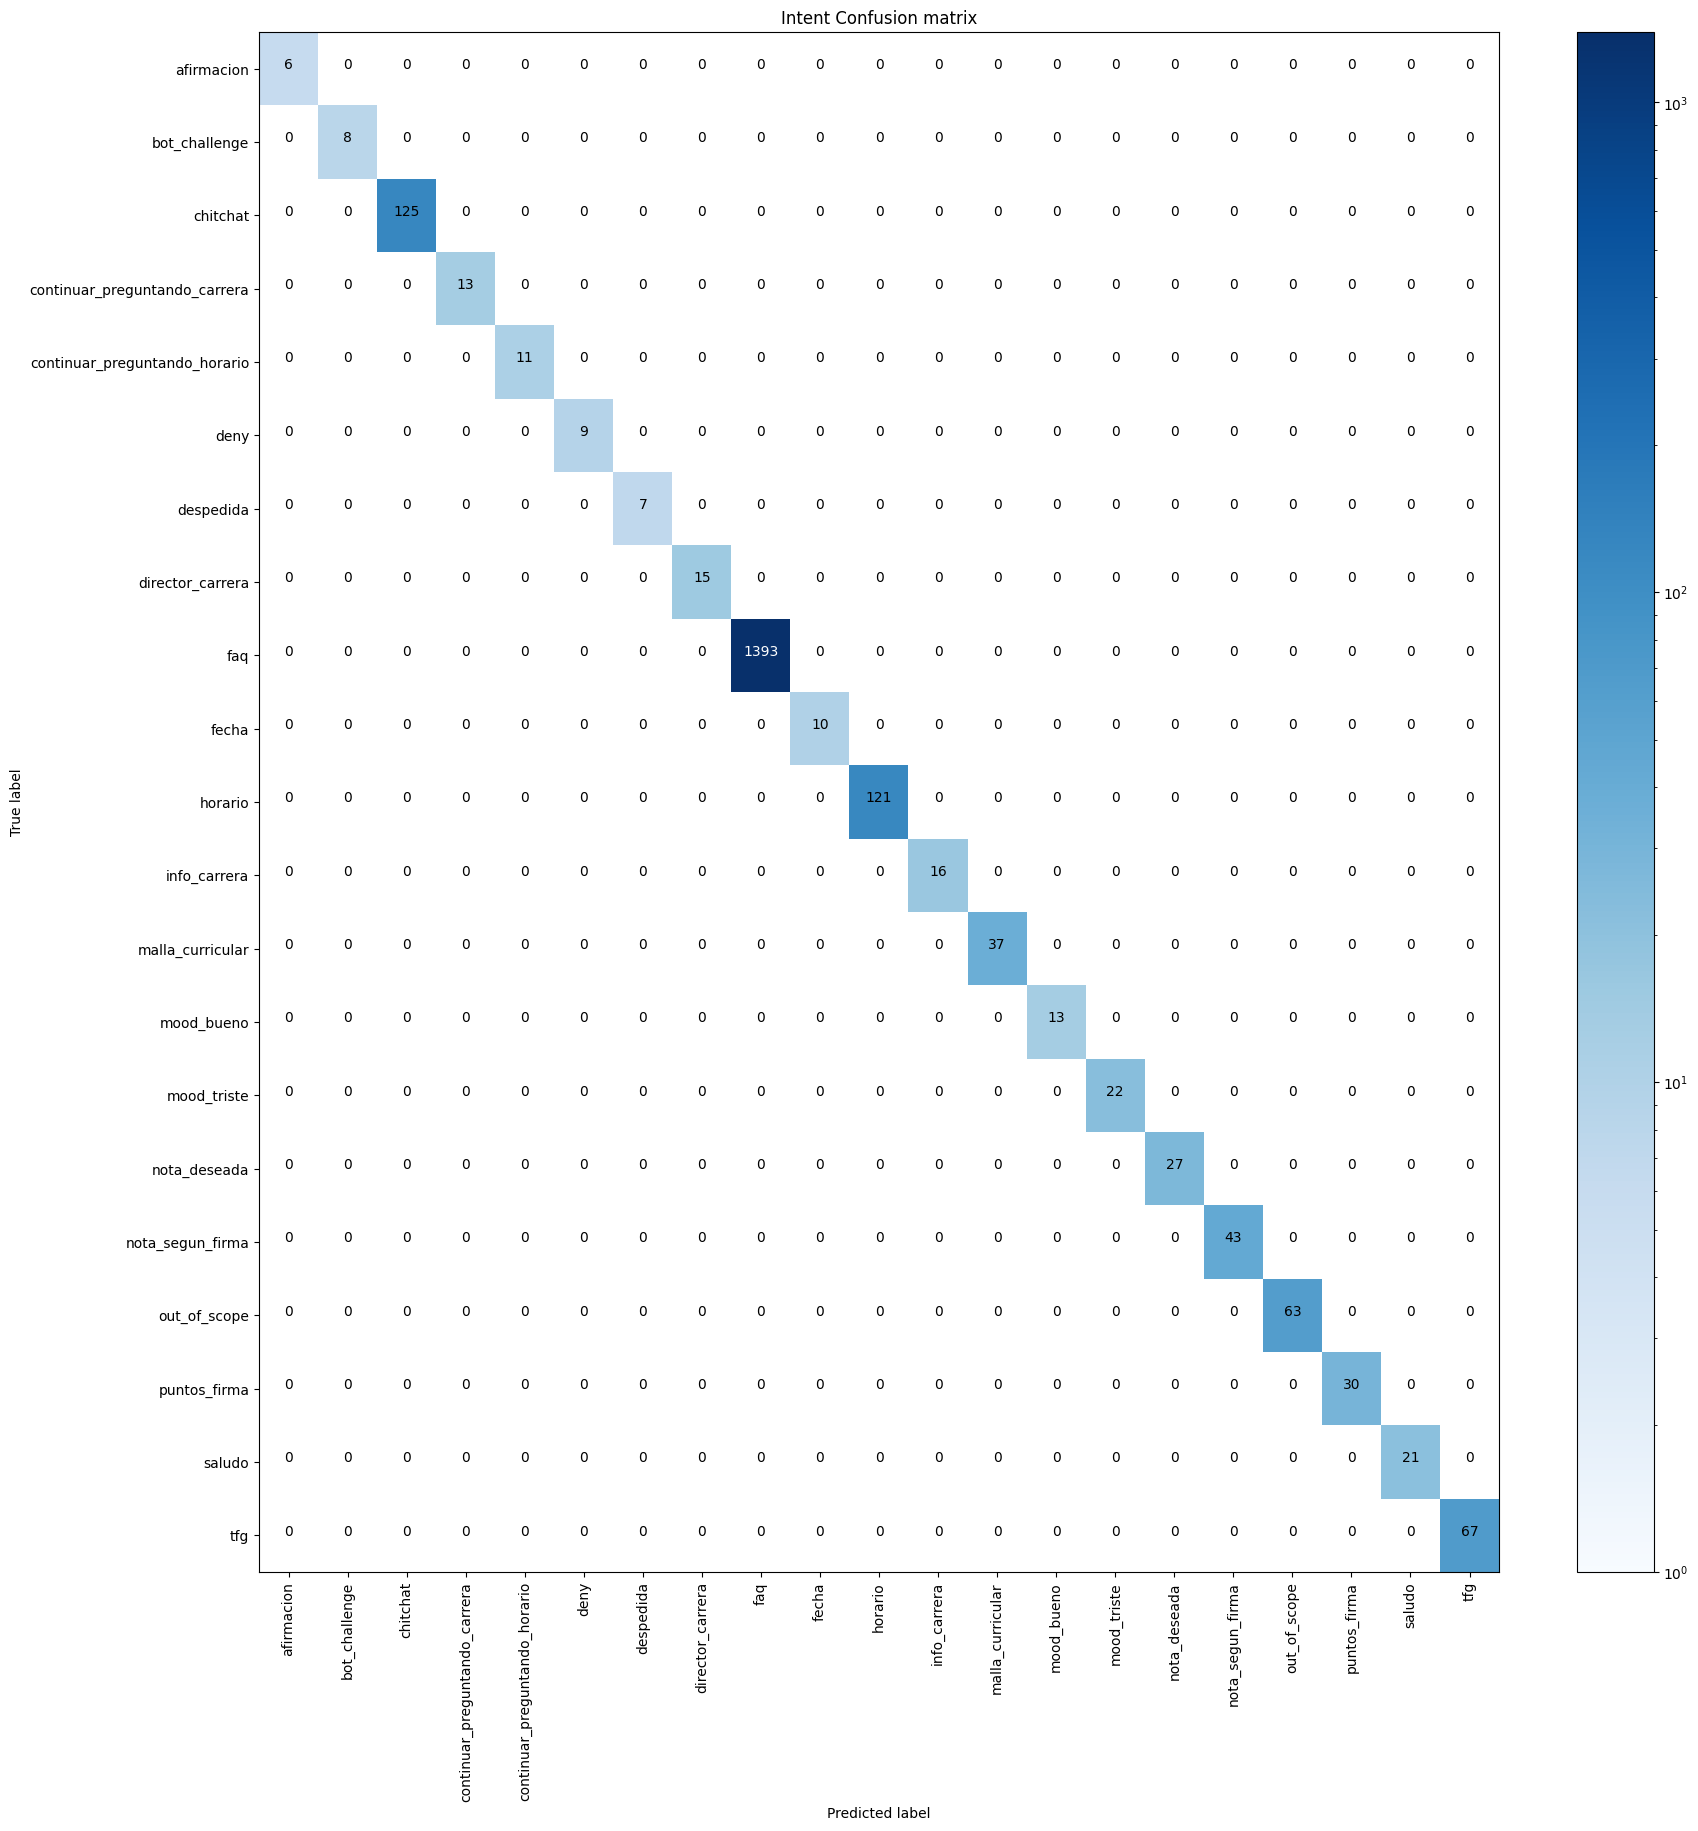
\includegraphics[width=\textwidth]{imagenes/cap5/intent_confusion_matrix.png}
	\caption{Matriz de Confusión de Intenciones}
	\label{fig:intent_matriz}
\end{figure}

\begin{figure}[H]
	\centering
	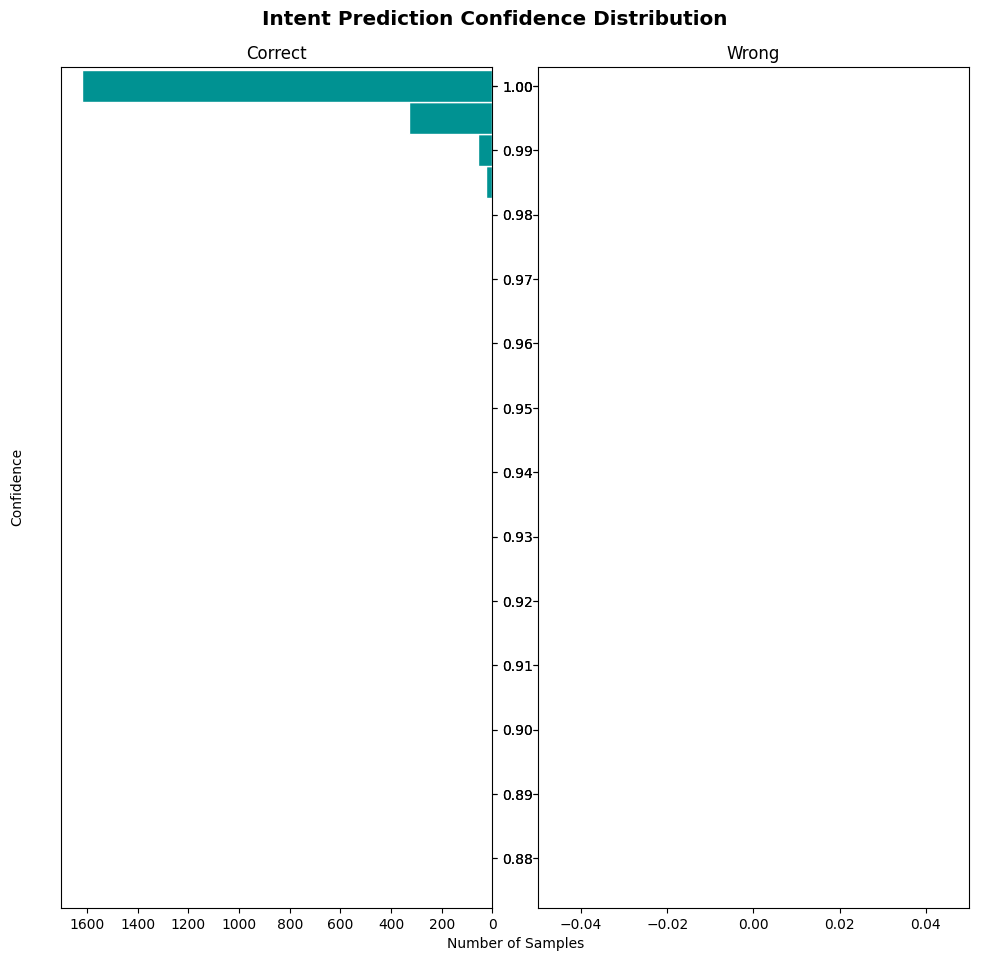
\includegraphics[width=\textwidth]{imagenes/cap5/intent_histogram.png}
	\caption{Histograma de confianza en la clasificación de Intenciones}
	\label{fig:intent_histograma}
\end{figure}

Al analizar la matriz de confusión \ref{fig:intent_matriz} y el histograma
\ref{fig:intent_histograma} podemos verificar que todas las intenciones fueron clasificadas
correctamente con una confianza superior a 0.98, indicando que el modelo es bastante efectivo en su
tarea de clasificación.
\subsection{Extracción de entidades}
Al ver los gráficos del extractor, tanto en la matriz de confusión de entidades
\ref{fig:entity_matriz} como en el histograma \ref{fig:entity_histograma} se encuentra que el
modelo se confunde con dos entidades, revisando el reporte de errores se encuentra que los
extractores DIETClassifier y EntitySynonymMapper reconocen las entidades por separado, esto genera
el error pero no afecta al rendimiento del modelo o a la correcta selección de una respuesta.

\begin{figure}[H]
	\centering
	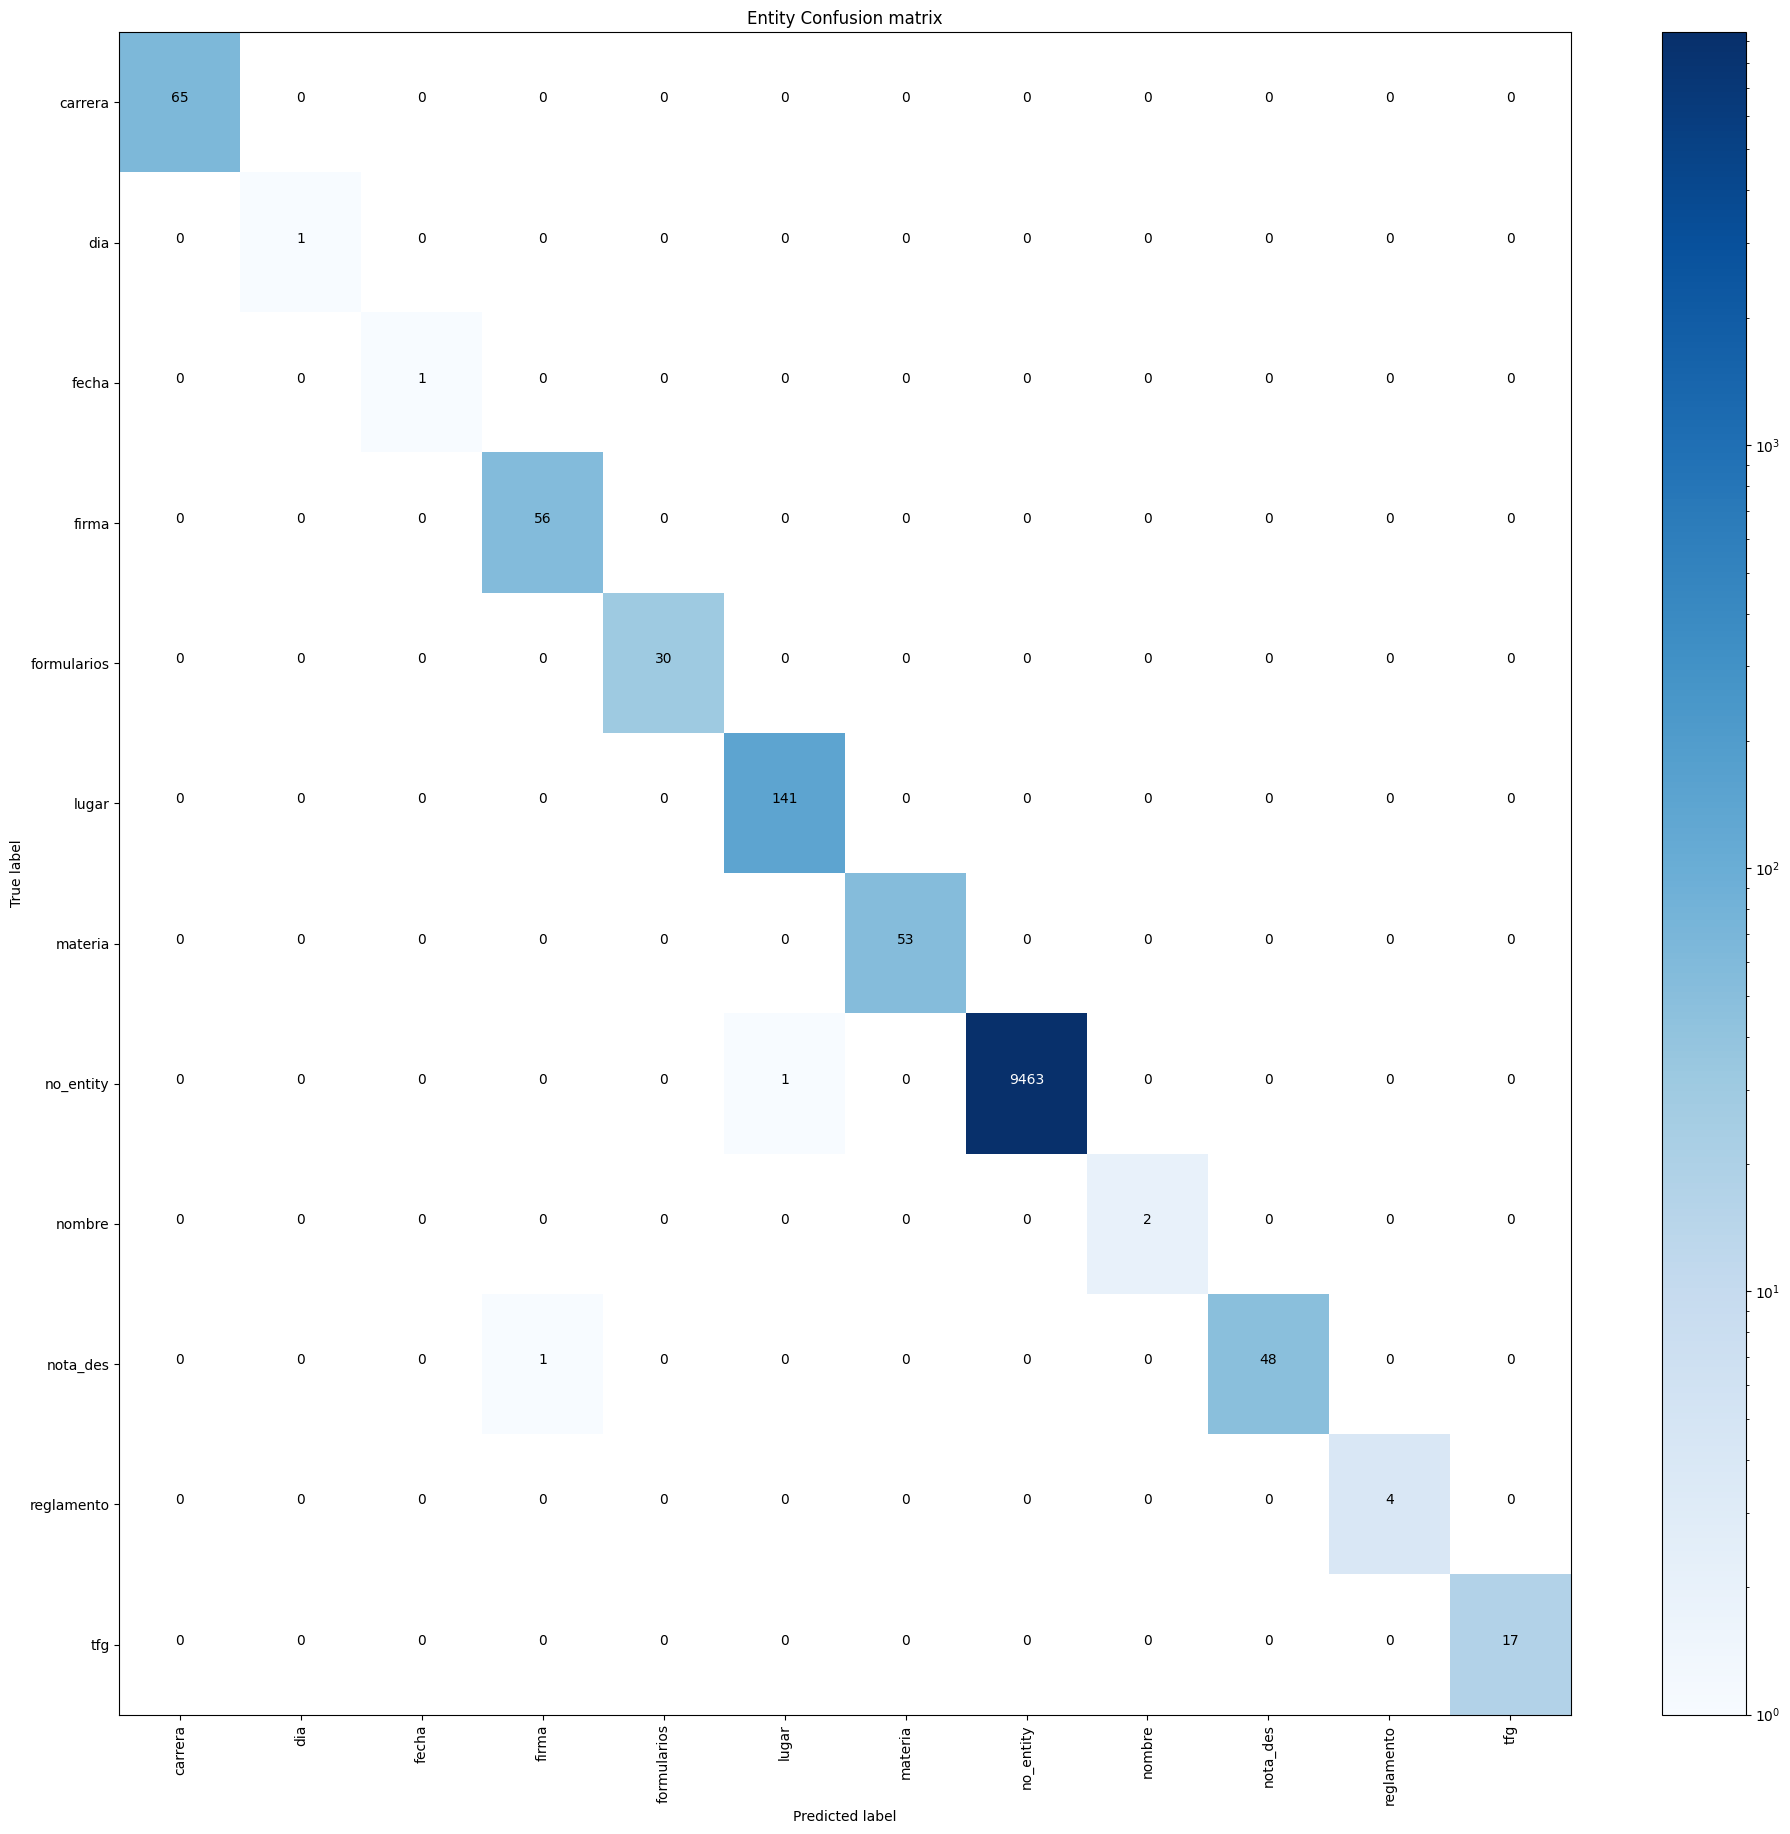
\includegraphics[width=\textwidth]{imagenes/cap5/DIETClassifier_confusion_matrix.png}
	\caption{Matriz de Confusión del extractor de entidades}
	\label{fig:entity_matriz}
\end{figure}

\begin{figure}[H]
	\centering
	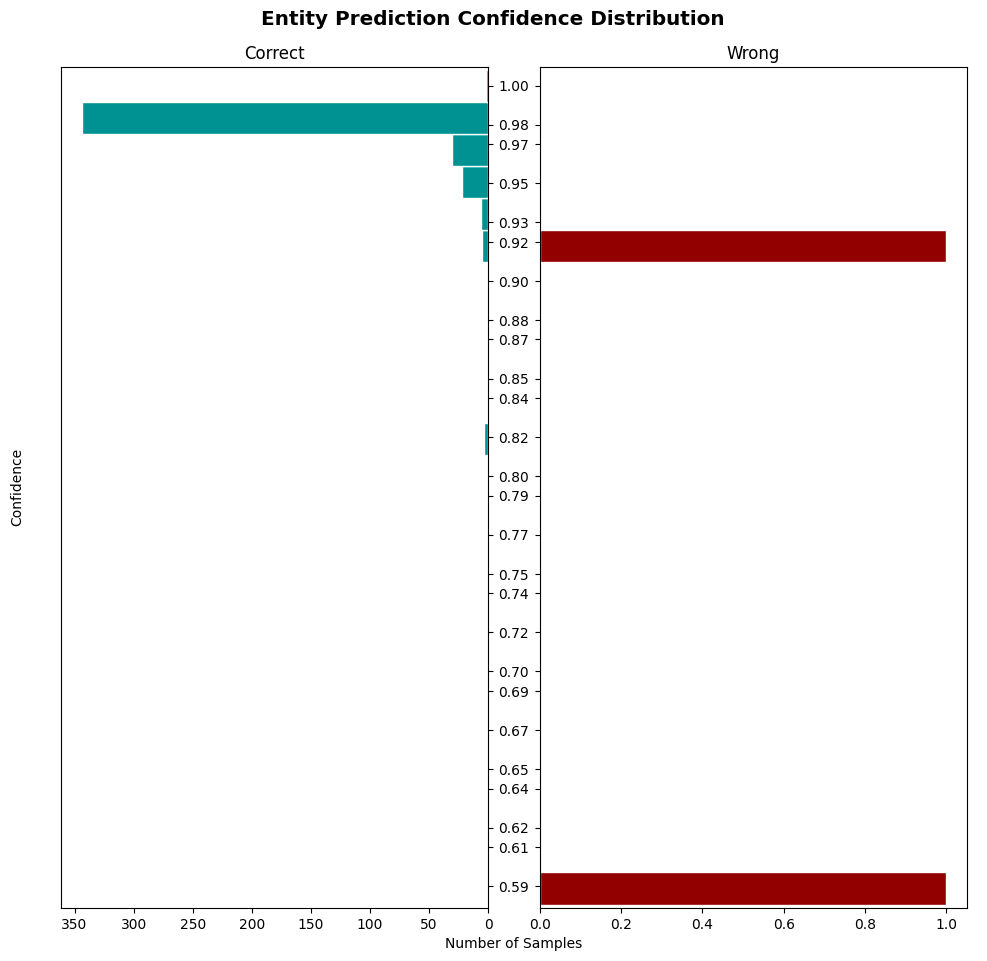
\includegraphics[width=\textwidth]{imagenes/cap5/DIETClassifier_histogram.png}
	\caption{Histograma de confianza del extractor de entidades}
	\label{fig:entity_histograma}
\end{figure}

\subsection{Selección de Respuestas}
Podemos observar en el histograma \ref{fig:response_histograma} de la selección de respuestas que
no se predijo erróneamente ninguna respuesta, la matriz de confusión en este caso no es de mucha
utilidad ya que son bastantes respuestas y complica la visibilidad de las etiquetas, en caso de que
existiese un error podremos encontrarlo en el reporte .json.

\begin{figure}[H]
	\centering
	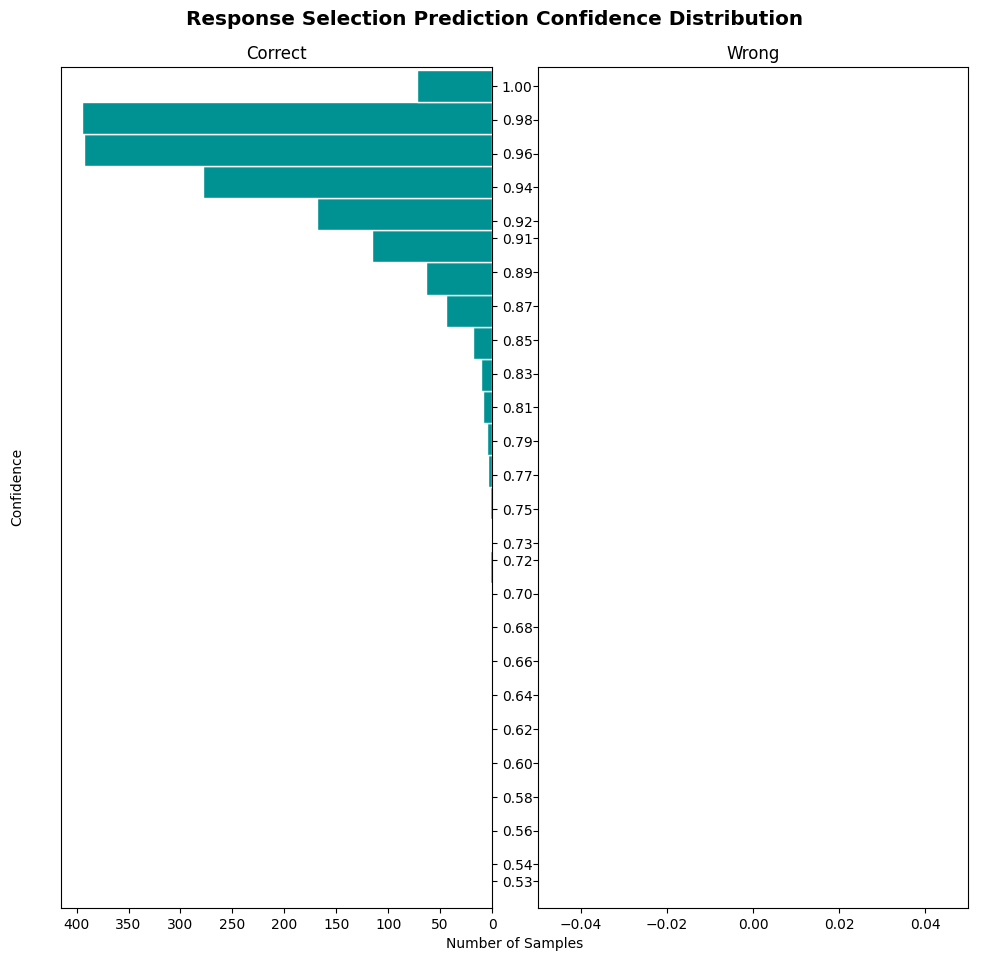
\includegraphics[width=\textwidth]{imagenes/cap5/response_selection_histogram.png}
	\caption{Histograma de confianza del seleccionador de respuestas}
	\label{fig:response_histograma}
\end{figure}

\section{Posibles Mejoras}
\begin{itemize}
	\item Integrar a sistemas existentes de la Facultad de Ingeniería.
	\item Se puede agregar respuestas de la chatbots públicos como	ChatGPT \cite{api_chatgpt}
	      para preguntas
	      fuera del
	      contexto de la Facultad de Ingeniería.
\end{itemize}
\chapter[Glosario]{Glosario}
\begin{itemize}
	\item \textbf{Acciones:} son funciones que se utilizan para realizar tareas en una conversación, pueden ser simples como respuestas genéricas o mas personalizadas con un código Python.
	\item \textbf{Aprendizaje Automático o de Máquina (Machine Learning):} es un subcampo de la inteligencia artificial que se enfoca en el desarrollo de algoritmos y modelos estadísticos que permiten a los sistemas informáticos aprender automáticamente de los datos, sin ser programados explícitamente para ello 
	\item \textbf{Aprendizaje Profundo (Deep Learning):} es una técnica de aprendizaje automático basada en redes neuronales artificiales de múltiples capas, que se utilizan para aprender patrones complejos y realizar tareas avanzadas como el reconocimiento de imágenes, voz y lenguaje natural.
	\item \textbf{Caracterizadores:} son herramientas de procesamiento de lenguaje natural que convierten texto en vectores numéricos utilizados para entrenar modelos de aprendizaje automático
	\item \textbf{Chatbot:} programas que imitan la conversación humana, capaces de interactuar con las personas y de responder adecuadamente a sus preguntas.
	\item \textbf{Conjunto de datos (Dataset):} es un conjunto de observaciones o ejemplos utilizados para entrenar modelos de aprendizaje automático
	\item \textbf{Contenedor:} forma de empaquetar y distribuir aplicaciones y sus dependencias junto con su configuración y recursos necesarios para su ejecución en diferentes entornos.
	\item \textbf{Docker:} plataforma de contenedores de software que permite empaquetar, distribuir y ejecutar aplicaciones y sus dependencias en entornos aislados.
	\item \textbf{Entidades:} representa un objeto o un concepto en una parte del texto, por ejemplo lugar o carrera.
	\item \textbf{Entorno Virtual:} herramienta que permite crear y gestionar un ambiente de trabajo aislado en un sistema operativo, con sus propias dependencias y configuraciones
	\item \textbf{Formularios:} son una manera de recopilar información necesaria para llevar a cabo una acción específica.
	\item \textbf{Intenciones:} en un mensaje del usuario, la intención es lo que se pretende transmitir o lograr
	\item \textbf{NLU:} se ocupa de analizar y comprender el lenguaje humano en un formato estructurado.
	\item \textbf{Procesamiento de Lenguaje Natural (NLP):} Campo de ciencias de Computación y la Lingüística que trata con métodos para analizar, modelar y entender el lenguaje humano.
	\item \textbf{Rasa Core:} forma parte de la librería Rasa, es el motor de diálogo que decide qué hacer a continuación en una conversación en función del contexto.
	\item \textbf{Rasa NLU:} es la parte de Rasa que realiza la comprensión del lenguaje natural (NLU), incluida la clasificación de intenciones y la extracción de entidades.
	\item \textbf{Reglas:} indica un comportamiento que se debe seguir en la conversación, donde una condición específica siempre predice una próxima acción específica.
	\item \textbf{Slots:} variables utilizadas para guardar información a lo largo de la conversación.
	\item \textbf{Tesauro:} vocabulario controlado y estructurado que se utiliza para indexar y recuperar información por medio de conceptos relacionados.
	\item \textbf{Tokenizadores:} herramienta utilizada en el procesamiento de lenguaje natural que divide el texto en unidades básicas de procesamiento de texto.
	\item \textbf{Transformadores:} tipo de arquitectura de redes neuronales utilizada en el procesamiento de lenguaje natural.
\end{itemize}

\chapter[CONCLUSIONES]{CONCLUSIONES}

\begin{itemize}
\item Revisamos las tecnologías y plataformas disponibles actualmente para el desarrollo de chatbots institucionales.
\item Se implementó un chatbot utilizando la plataforma Rasa OpenSource, el cual responde preguntas frecuentes de los estudiantes de la Facultad de Ingeniería.
\item Se utilizó un dataset inicial propio y se recopilaron preguntas de los alumnos en grupos de prueba para entrenar el modelo.
\item Seleccionamos, entrenamos y probamos el algoritmo utilizando el dataset generado.
\item Entrenamos y probamos el modelo a partir de los datos recopilados.
\item Se implementó un servidor público que alberga los servicios del chatbot.
\item Se utilizó la API de Telegram para que el chatbot esté disponible para los alumnos de la Facultad de Ingeniería.
\end{itemize}

%%%bibliografía%%%%%%%%%
%Cargar los libros en formato bibtex en el archivo fiuna.bib
\formatoIndice
\bibliographystyle{fiuna}
%\nocite{*}
\bibliography{fiuna}   

%%%anexos%%%%%%
%En caso de no tenerlos, comentar la siguiente línea
\appendixpageoff
\begin{appendices}
%Agregar los apéndices

\chapter*{Anexo A: Comandos de Rasa}
\addcontentsline{loa}{appendix}{Anexo A: Comandos de Rasa}
% Please add the following required packages to your document preamble:
% \usepackage{multirow}
% \usepackage{graphicx}
\begin{table}[h]
\resizebox{\textwidth}{!}{%
\begin{tabular}{|l|l|l}
\cline{1-2}
\multicolumn{1}{|c|}{\textbf{Comando}} & \multicolumn{1}{c|}{\textbf{Efecto}}                                                                                                    &  \\ \cline{1-2}
\multirow{2}{*}{rasa init}             & \multirow{2}{*}{Crea un nuevo proyecto con un ejemplo de entrenamiento, acciones y archivos de configuracion.}                          &  \\
                                       &                                                                                                                                         &  \\ \cline{1-2}
\multirow{2}{*}{rasa train}            & \multirow{2}{*}{Entrena un modelo utilizando datos NLU y lo guarda en ./models.}                                                        &  \\
                                       &                                                                                                                                         &  \\ \cline{1-2}
\multirow{2}{*}{rasa interactive}      & \multirow{2}{*}{Empieza una sesion interactiva de aprendizaje para crear un dataset nuevo de entrenamiento, chateando con el asistente} &  \\
                                       &                                                                                                                                         &  \\ \cline{1-2}
\multirow{2}{*}{rasa shell}            & \multirow{2}{*}{Carga el modelo entrenado y permite conversar con tu asistente en la linea de comando}                                   &  \\
                                       &                                                                                                                                         &  \\ \cline{1-2}
\multirow{2}{*}{rasa run}              & \multirow{2}{*}{Inicia un servidor con el modelo entrenado}                                                                             &  \\
                                       &                                                                                                                                         &  \\ \cline{1-2}
\multirow{2}{*}{rasa run actions}      & \multirow{2}{*}{Inicia un servidor de acciones utiliando el SDK de Rasa}                                                                &  \\
                                       &                                                                                                                                         &  \\ \cline{1-2}
\multirow{2}{*}{rasa visualize}        & \multirow{2}{*}{Genera una representación visual de las historias}                                                                      &  \\
                                       &                                                                                                                                         &  \\ \cline{1-2}
\multirow{2}{*}{rasas test}            & \multirow{2}{*}{Prueba un modelo entrenado de Rasa en cualquier archivo que empiea con test\_.}                                         &  \\
                                       &                                                                                                                                         &  \\ \cline{1-2}
\multirow{2}{*}{rasas data split nlu}  & \multirow{2}{*}{Realiza una separacion 80/20 de los datos de entrernamiento}                                                            &  \\
                                       &                                                                                                                                         &  \\ \cline{1-2}
\multirow{2}{*}{rasa data convert}     & \multirow{2}{*}{Convierte los datos de entrenamiento entre diferentes formatos}                                                         &  \\
                                       &                                                                                                                                         &  \\ \cline{1-2}
\multirow{2}{*}{rasa data migrate}     & \multirow{2}{*}{Migra del dominio 2.0 al formato 3.0}                                                                                   &  \\
                                       &                                                                                                                                         &  \\ \cline{1-2}
\multirow{2}{*}{rasa data validate}    & \multirow{2}{*}{Controla que los datos del  dominio, de la NLU y de la conversación no sean incoherentes}                               &  \\
                                       &                                                                                                                                         &  \\ \cline{1-2}
\multirow{2}{*}{rasa export}           & \multirow{2}{*}{Exporta conversaciones de un almacén de seguimiento a un corredor de eventos.}                                          &  \\
                                       &                                                                                                                                         &  \\ \cline{1-2}
\multirow{2}{*}{rasa valuates markers} & \multirow{2}{*}{Extrae los marcadores de un almacén de seguimiento existente.}                                                          &  \\
                                       &                                                                                                                                         &  \\ \cline{1-2}
\multirow{2}{*}{rasa x}                & \multirow{2}{*}{Inicia Rasa X en modo local}                                                                                            &  \\
                                       &                                                                                                                                         &  \\ \cline{1-2}
\multirow{2}{*}{rasa -h}               & \multirow{2}{*}{Muestra los comandos disponibles}                                                                                       &  \\
                                       &                                                                                                                                         &  \\ \cline{1-2}
\end{tabular}%
}
\end{table}


\chapter*{Anexo B: El uso de plantillas}
\addcontentsline{loa}{appendix}{Anexo B: El uso de plantillas}

Aquí el contenido del anexo B



\end{appendices}
\end{document}
